%%==================================================
%% chapter01.tex for BIT Master Thesis
%% modified by pinren lu
%% version: 0.1
%% last update: Dec 25th, 2016
%%==================================================

\chapter{模型改写文本检测方法}
\label{chap:method}

\section{引言}
\label{sec:method-intro}

在第三章中,我们详细介绍了模型改写文本检测数据集(TOSWT 数据集)的构造方法,强调了数据清洗、句子分割以及利用大型语言模型进行文本改写的重要性。这一过程为后续的文本检测任务奠定了坚实的基础。在本章中,我们将深入探讨模型改写文本检测的方法,着重分析基于预训练模型的技术路线,并阐明实验设计及其结果。

随着人工智能技术的飞速发展,尤其是大型语言模型的广泛应用,文本生成的质量和复杂性显著提升。这使得传统的文本检测方法面临新的挑战,尤其是在识别和追踪人工智能生成文本方面。因此,开发有效的模型改写文本检测方法,成为了当前自然语言处理领域的重要研究方向。通过构建有效的检测模型,我们能够更好地识别出文本中可能的人工智能生成部分,从而为教育领域提供支持。

本章的核心目标是介绍两种基于预训练模型的文本检测方法,分别是 RoBERTa 和 DeBERTa 先进的语言模型。这些模型在自然语言理解和生成任务中表现出色,能够通过深层次的语义理解来识别文本的来源。我们将分析这些模型的架构和训练过程,并探讨它们在文本检测任务中的具体应用。

此外,我们将设计一系列实验,以评估所提出的方法在模型改写文本检测中的有效性。这些实验将包括数据集设置、参数配置、评价指标的选择以及对比实验和消融实验的结果分析。通过这些实验,我们不仅能够验证所提出方法的性能,还能为后续研究提供宝贵的经验和数据支持。

本章的结构安排如下:首先,我们将介绍基于预训练的模型改写文本检测方法,详细分析 RoBERTa 和 DeBERTa 模型的特点和应用。接着,我们将阐述实验设计,包括数据集的设置、实验参数的配置以及评价指标的选择。最后,我们将对实验结果进行深入分析,以评估所提出方法的有效性和实用性。

通过本章的研究,我们希望能够为模型改写文本检测领域提供新的思路和方法,推动相关技术的发展与应用。同时,我们也期待这些研究成果能够为教育工作者提供切实可行的解决方案,并启发内容审核人员以及其他相关领域的从业者的应用思路,以应对日益复杂的文本来源问题。

\section{基于预训练的模型改写文本检测方法}
\label{sec:method-pretrain}

随着自然语言处理(NLP)技术的不断进步,基于预训练模型的方法在文本分析和理解任务中取得了显著的成功。预训练模型通过在大量文本数据上进行训练,学习到丰富的语言特征和语义信息,这使得它们在特定任务中表现出色。在模型改写文本检测领域,利用这些预训练模型能够有效地识别和追踪文本的来源,尤其是在面对人工智能生成的文本时。

预训练模型的核心优势在于其强大的上下文理解能力。与传统的特征工程方法相比,预训练模型能够自动提取文本中的深层次特征,从而提高文本分类和检测的准确性。这一过程通常分为两个阶段:首先是在大规模文本数据上进行无监督预训练,然后在特定任务上进行微调。通过这种方式,模型能够适应不同的文本风格和结构,从而增强其在特定应用场景下的性能。

在模型改写文本检测任务中,预训练模型的使用能够帮助我们识别文本中的细微差异,例如句子结构的变化、用词的替换以及语义的调整。这对于判断文本是否经过人工智能模型的改写尤为重要。通过分析文本的上下文信息,预训练模型能够捕捉到潜在的模式和特征,这些模式可能是人类作者与人工智能生成文本之间的显著区别。

在本节中,我们将介绍两种流行且被本课题应用的预训练模型:RoBERTa \cite{liu_roberta_2019} 和 DeBERTa \cite{he_deberta_2021, he2023debertav3improvingdebertausing}。这两种模型在文本理解和生成任务中都表现出色,尤其是在文本分类和检测方面,已被广泛应用于多个研究领域。

%%% TODO: 把下面的 RoBERTa 和 DeBERTa 统统丢进去润色一遍!

\subsection{RoBERTa 模型}
\label{sec:method-pretrain-roberta}

RoBERTa \cite{liu_roberta_2019}(Robustly Optimized BERT Approach)在 BERT \cite{devlin_bert_2019} 模型的基础上进行了多方面的改进,从而显著提升了模型的性能。

在训练策略方面,原始的 BERT 模型存在训练不足的问题。为了解决这一问题,RoBERTa 通过延长训练步数、使用更大的批次进行训练,并在更广泛的数据集上进行训练。在实验中,使用更大的批次训练 BERT 模型的结果表明,这种方法能够有效改善训练的困惑度(perplexity)和下游任务的准确率。此外,大批次训练更易于通过分布式数据并行训练实现,从而提高了训练效率。

在训练数据的选择上,RoBERTa 使用了包含多种语料库的总计 160GB 未压缩文本,这一数据量远超 BERT 原始训练所用的 16GB 数据。这一结果充分验证了数据量和多样性在预训练过程中所起的重要作用。同时,BERT 原始实现中,掩码是在数据预处理阶段一次性生成的,形成了静态掩码。尽管通过复制数据来增加掩码的多样性,但这种方法仍存在局限性。相较之下,RoBERTa 采用了动态掩码机制,即每次向模型输入序列时都生成新的掩码模式。这一方法在长时间训练或处理大规模数据集时表现出明显的优势,不仅提升了训练效率,还在实验中显示出相较于静态掩码更优或相当的性能。

在模型输入格式的优化上,原始 BERT 模型在训练时使用了下一个句子预测(NSP)任务,旨在提升下游任务的性能。然而,当时的一些研究 \cite{Lample2019CrosslingualLM, Yang2019XLNetGA, Joshi2019SpanBERTIP} 对这一任务提出了质疑。经过对比实验,RoBERTa 发现去除 NSP 损失并采用从单个文档中采样完整句子作为输入能够匹配或略微提升下游任务的性能。具体而言,限制序列来自单个文档的 DOC-SENTENCES 格式表现稍好于从多个文档打包的 FULL-SENTENCES 格式,但为了便于与相关研究的比较,最终 RoBERTa 采用了从多个文档打包的 FULL-SENTENCES 格式。此外,RoBERTa 不再使用 BERT 原有的两文档片段拼接并添加 NSP 损失的输入格式,而是采用了从一个或多个文档中连续采样完整句子的方式,使得输入总长度不超过 512 个标记。这一格式有助于模型学习长距离依赖关系,从而增强了文本理解的能力。

在文本编码的改进方面,BERT 原实现使用了一个大小为 30K 的字符级字节对编码 \cite{BPE} (BPE)词汇表,并需要进行启发式分词规则的预处理。RoBERTa 借鉴了其他研究,采用了一个包含 50K 子词单元的更大字节级 BPE 词汇表,这一方法无需额外的预处理或分词。尽管在部分任务上性能略有下降,但由于其通用编码方案的优势,RoBERTa 仍被广泛应用于后续的实验中。

通过上述基于 BERT 的改进,RoBERTa 在多个自然语言处理任务中展现出了卓越的性能,为后续研究提供了强有力的支持。

在本文中,采用 RoBERTa-base 和 RoBERTa-Large 两种大小的 RoBERTa 模型,其参数如表 \ref{tab:roberta-parameter} 所示。表中的参数包括 Transformer 层数、隐藏层维度、注意力头数以及总参数量。这些参数的设计反映了模型的复杂性及其学习能力。较大的模型(RoBERTa-Large)在处理更复杂的语言任务时,能够更好地捕捉深层次的语义关系和上下文信息,而较小的模型(RoBERTa-Base)则在计算效率和资源消耗上具有一定的优势。通过对比这两种模型的性能,我们能够深入探讨不同规模模型在文本理解和生成任务中的表现差异,从而为后续研究提供有价值的参考。

\begin{table*}[htbp]
\centering
\caption{ RoBERTa-Base 和 RoBERTa-Large 参数} \label{tab:roberta-parameter}
\begin{tabular}{lcc}
\toprule
               & \multicolumn{1}{l}{\textbf{RoBERTa-Base}} & \multicolumn{1}{l}{\textbf{RoBERTa-Large}} \\ \midrule
Transformer 层数 & 12                                        & 24                                         \\
隐藏层维度          & 768                                       & 1024                                       \\
注意力头数          & 12                                        & 16                                         \\
总参数量           & 125M                                      & 355M                                      \\ \bottomrule
\end{tabular}
\end{table*}

\subsection{DeBERTa 模型}
\label{sec:method-pretrain-deberta}

目前 DeBERTa 系列模型公开的论文仅有 DeBERTa 模型 \cite{he_deberta_2021} 和 DeBERTa V3 模型 \cite{he2023debertav3improvingdebertausing},我们的实验中将会使用 DeBERTa V3 模型,本节将会对 DeBERTa 模型对于 BERT \cite{devlin_bert_2019} 和 RoBERTa 模型 \cite{liu_roberta_2019} 的改进进行介绍。

\subsubsection{DeBERTa 模型}

DeBERTa 模型 \cite{he_deberta_2021} 是预训练语言模型不断演进过程中的佼佼者,相较于RoBERTa和BERT有诸多显著改进。这些改进主要体现在注意力机制、掩码解码器以及训练方法等方面,使其在模型性能和泛化能力上都有大幅提升。

在注意力机制方面,BERT和RoBERTa在输入层将每个单词表示为其词嵌入(内容)与位置嵌入之和的向量,这种表示方式在一定程度上混合了内容和位置信息。而DeBERTa创新性地采用解耦注意力机制,每个单词由两个独立向量分别编码内容和位置。在计算单词间注意力权重时,DeBERTa使用基于内容和相对位置的解耦矩阵分别计算,通过这种方式,能更精细地捕捉单词之间的关系。以句子 “The dog chased the cat” 为例,当分析 “dog” 和 “cat” 的关系时,不仅考虑它们的语义内容,还能依据相对位置更准确地判断其依赖关系,相比之下,BERT和RoBERTa难以如此细致地处理这种关系。

对于序列中位置为 $i$ 的一个词元(token),DeBERTa 用两个向量 $\mathbf{H}_{i}$ 和 $\mathbf{P}_{i|j}$ 来表示它,其中 $\mathbf{H}_{i}$ 代表该词元的内容,$\mathbf{P}_{i|j}$  代表它与位置为 $j$ 的词元的相对位置。词元 $i$ 和 $j$ 之间的交叉注意力分数的计算可以分解为四个部分,即:
\begin{align}
\label{eq:deberta-attention}
\begin{split}
\mathbf{A}_{i, j} & = \{\mathbf{H}_{i}, \mathbf{P}_{i | j}\} \times \{\mathbf{H}_{j}, \mathbf{P}_{j | i}\}^{\intercal} \\
& = \mathbf{H}_{i}\mathbf{H}_{j}^{\intercal}+\mathbf{H}_{i}\mathbf{P}_{j | i}^{\intercal}+\mathbf{P}_{i | j}\mathbf{H}_{j}^{\intercal}+\mathbf{P}_{i | j}\mathbf{P}_{j | i}^{\intercal}.
\end{split}
\end{align}

也就是说,一对单词的注意力权重可以通过使用基于它们的内容和位置的解耦矩阵,将四个注意力分数相加来计算,这四个分数分别为内容对内容、内容对位置、位置对内容以及位置对位置的注意力分数。

而在 DeBERTa 之前的相对位置编码方法在计算注意力权重时,使用单独的嵌入矩阵来计算相对位置偏差 \cite{Shaw2018SelfAttentionWR, Huang2018MusicTG}。这相当于仅使用公式 \ref{eq:deberta-attention} 中的内容对内容和内容对位置项来计算注意力权重。DeBERTa 模型认为位置对内容这一项也很重要,因为一对单词的注意力权重不仅取决于它们的内容,还取决于它们的相对位置,而只有同时使用内容对位置和位置对内容项才能对其进行全面建模。由于 DeBERTa 使用相对位置嵌入,位置对位置项不会提供太多额外信息,因此在我们的实现中从公式 \ref{eq:deberta-attention} 中去掉了该项。

以单头注意力为例,标准的自注意力操作 \cite{transformer} 可以表示为:
\begin{align}
\mathbf{Q} = \mathbf{HW_{q}}, \mathbf{K} &= \mathbf{HW_{k}}, V = \mathbf{HW_{v}}, \mathbf{A} = \frac{\mathbf{QK}^{\intercal}}{\sqrt{d}} \\
\mathbf{H_{o}} &= \text{softmax}(\mathbf{A})\mathbf{V}
\label{eq:transformer-attention1}
\end{align}
其中,$\mathbf{H} \in \mathbb{R}^{N×d}$ 表示输入的隐藏向量,$\mathbf{H_{o}} \in \mathbb{R}^{N×d}$ 是自注意力的输出,$\mathbf{W_{q}}$、$\mathbf{W_{k}}$、$\mathbf{W_{v}} \in \mathbb{R}^{d×d}$ 是投影矩阵,$\mathbf{A} \in \mathbb{R}^{N×N}$ 是注意力矩阵,$N$ 是输入序列的长度,$d$ 是隐藏状态的维度。

记 $k$ 为最大相对距离,$\delta(i, j) \in [0, 2k)$ 为从词元 $i$ 到词元 $j$ 的相对距离,其定义为:
\begin{align}
\delta(i, j)=\begin{cases}
0, & \text{当~} i - j \leq -k \\
2k - 1, & \text{当~} i - j \geq k \\
i - j + k, & \text{其他情况}
\end{cases}
\label{eq:deberta-distance}
\end{align}

DeBERTa 中将带有相对位置偏差的解耦自注意力表示为公式 \ref{eq:deberta-dis-att},其中 $\mathbf{Q}_{c}$、$\mathbf{K}_{c}$ 和 $\mathbf{V}_{c}$ 是分别使用投影矩阵 $\mathbf{W}_{q,c}$、$\mathbf{W}_{k,c}$、$\mathbf{W}_{v,c} \in \mathbb{R}^{d×d}$ 生成的投影内容向量。$\mathbf{P} \in \mathbb{R}^{2k×d}$ 表示在所有层中共享的相对位置嵌入向量(即在正向传播过程中保持固定),$\mathbf{Q}_{r}$ 和 $\mathbf{K}_{r}$ 是分别使用投影矩阵 $\mathbf{W}_{q,r}$、$\mathbf{W}_{k,r} \in \mathbb{R}^{d×d}$ 生成的投影相对位置向量。
\begin{align} \label{eq:deberta-dis-att}
\begin{split}
    \mathbf{Q}_c = \mathbf{H} \mathbf{W}_{q,c}, 
    \mathbf{K}_c &= \mathbf{H} \mathbf{W}_{k,c}, 
    \mathbf{V}_c = \mathbf{H} \mathbf{W}_{v,c}, 
    \mathbf{Q}_r = \mathbf{P} \mathbf{W}_{q,r}, 
    \mathbf{K}_r = \mathbf{P} \mathbf{W}_{k,r} \\
    \tilde{\mathbf{A}}_{i,j} &= \underbrace{\mathbf{Q}^{c}_{i}{\mathbf{K}^{c}_{j}}^{\intercal}}_{\text{(a) content-to-content}}  
    + \underbrace{\mathbf{Q}^{c}_{i}{{\mathbf{K}^{r}_{\delta(i,j)}}^{\intercal}}}_{\text{(b) content-to-position}}
    + \underbrace{\mathbf{K}^{c}_{j}{{\mathbf{Q}^{r}_{\delta(j,i)}}^{\intercal}}}_{\text{(c) position-to-content}} \\
    \mathbf{H_o} &= \text{softmax}(\frac{\tilde{\mathbf{A}}}{\sqrt{3d}})\mathbf{V}_c
\end{split}
\end{align}
$\tilde{\mathbf{A}}_{i, j}$ 是注意力矩阵 $\tilde{\mathbf{A}}$ 的元素,表示从词元 $i$ 到词元 $j$ 的注意力分数。$\mathbf{Q}_{i}^{c}$ 是 $\mathbf{Q}_{c}$ 的第 $i$ 行,$\mathbf{K}_{j}^{c}$ 是 $\mathbf{K}_{c}$ 的第 $j$ 行,$\mathbf{K}_{\delta(i, j)}^{r}$ 是 $\mathbf{K}_{r}$ 中与相对距离 $\delta(i, j)$ 对应的第 $\delta(i, j)$ 行,$\mathbf{Q}_{\delta(j, i)}^{r}$ 是 $\mathbf{Q}_{r}$ 中与相对距离 $\delta(j, i)$ 对应的第 $\delta(j, i)$ 行。注意这里我们使用 $\delta(j, i)$ 而不是 $\delta(i, j)$,这是因为对于给定的位置 $i$,位置对内容计算的是位置 $j$ 处的键内容相对于位置 $i$ 处的查询位置的注意力权重,因此相对距离是 $\delta(j, i)$。位置对内容项的计算为 $\mathbf{K}_{j}^{c}{\mathbf{Q}_{\delta(j, i)}^{r}}^{\intercal}$,内容对位置项的计算方式类似。

最后,我们对 $\tilde{\mathbf{A}}$ 应用一个缩放因子 $\frac{1}{\sqrt{3d}}$。这个因子对于稳定模型训练很重要 \cite{transformer},特别是对于大规模预训练语言模型。

\begin{algorithm}[htbp]
\caption{解耦注意力(Disentangled Attention)}
\label{algo:DA}
%\SetAlgoLined
 \begin{algorithmic}[1]
    \Require {隐藏状态 $\mathbf{H}$, 相对距离嵌入 $\mathbf{P}$, 相对距离矩阵 $\mathbf{\delta}$.}
    内容投影矩阵 $\mathbf{W}_{k,c}$, $\mathbf{W}_{q,c}$, $\mathbf{W}_{v,c}$,
    位置投影矩阵 $\mathbf{W}_{k,r}$, $\mathbf{W}_{q,r}$.
    \Ensure $\mathbf{H}_o$

    \State {$\mathbf{K}_c = \mathbf{H}\mathbf{W}_{k,c}$, $\mathbf{Q}_c = \mathbf{H}\mathbf{W}_{q,c}$, $\mathbf{V}_c = \mathbf{H}\mathbf{W}_{v,c}$,   $\mathbf{K}_r = \mathbf{P}\mathbf{W}_{k,r}$, $\mathbf{Q}_r = \mathbf{P}\mathbf{W}_{q,r}$}
    \State {$\mathbf{A}_{c\rightarrow c} = \mathbf{Q}_c \mathbf{K}_c^{\intercal}$} 
    \For{$i=0,...,N-1$} 
        \State {$\tilde{\mathbf{A}}_{c\rightarrow p}[i,:] = \mathbf{Q}_{c}[i,:] \mathbf{K}_r^{\intercal}$} 
    \EndFor
    \For {$i=0,...,N-1$}
        \For {$j=0,...,N-1$}
        \State {$\mathbf{A}_{c\rightarrow p}[i,j] = \tilde{\mathbf{A}}_{c\rightarrow p}[i,\mathbf{\delta}[i,j]]$} 
        \EndFor
    \EndFor
    \For{$j=0,...,N-1$}
        \State {$\tilde{\mathbf{A}}_{p\rightarrow c}[:,j] = \mathbf{K}_{c}[j,:] \mathbf{Q}_r^{\intercal}$} 
    \EndFor
    \For {$j=0,...,N-1$}
        \For {$i=0,...,N-1$}
        \State {$\mathbf{A}_{p\rightarrow c}[i,j] = \tilde{\mathbf{A}}_{p\rightarrow c}[\mathbf{\delta}[j,i],j]$} 
        \EndFor
    \EndFor
    \State {$\tilde{\mathbf{A}}=\mathbf{A}_{c\rightarrow c} + \mathbf{A}_{c\rightarrow p} + \mathbf{A}_{p\rightarrow c}$}
    \State {$\mathbf{H}_o = \text{softmax}(\frac{\tilde{\mathbf{A}}}{\sqrt{3d}})\mathbf{V}_c$}
 \end{algorithmic}

\end{algorithm}

DeBERTa 中采取了一种高效实现。在 DeBERTa 之前的研究中对于长度为 $N$ 的输入序列,存储每个词元的相对位置嵌入需要 $O(N^{2}d)$ 的空间复杂度 \cite{Shaw2018SelfAttentionWR, Huang2018MusicTG, Dai2019TransformerXLAL}。然而,以内容对位置为例,DeBERTa 中注意到由于 $\delta(i, j) \in [0, 2k)$,并且所有可能相对位置的嵌入始终是 $\mathbf{K}_{r} \in \mathbb{R}^{2k×d}$ 的一个子集,因此我们可以在所有查询的注意力计算中重用 $\mathbf{K}_{r}$。

在 DeBERTa 中,预训练时将最大相对距离 $k$ 设置为512。解耦注意力权重可以使用算法 \ref{algo:DA} 高效计算。令 $\delta$ 为根据公式 \ref{eq:deberta-distance} 得到的相对位置矩阵,即 $\delta[i, j] = \delta(i, j)$。我们不是为每个查询分配不同的相对位置嵌入矩阵,而是将每个查询向量 $\mathbf{Q}_{c}[i, :]$ 乘以 $\mathbf{K}_{r}^{\intercal} \in R^{d×2k}$(如算法 \ref{algo:DA} 的第 3-5 行),然后使用相对位置矩阵 $\delta$ 作为索引提取注意力权重(如算法 \ref{algo:DA} 的第 6-10 行)。为了计算位置对内容的注意力分数,我们通过将每个键向量 $\mathbf{K}_{c}[j, :]$ 乘以 $\mathbf{Q}_{r}^{T}$ 来计算 $\tilde{\mathbf{A}}_{p \to c}[:, j]$,即注意力矩阵 $\tilde{\mathbf{A}}_{p \to c}$ 的列向量(如算法 \ref{eq:deberta-distance} 的第 11-13 行),最后通过相对位置矩阵 $\delta$ 作为索引提取相应的注意力分数(如算法1的第14 - 18行)。通过这种方式,我们不需要为每个查询分配内存来存储相对位置嵌入,从而将空间复杂度降低到 $O(kd)$(用于存储 $\mathbf{K}_{r}$ 和 $\mathbf{Q}_{r}$)。 

除此之外,DeBERTa 还采用掩码语言建模(Masked Language Modeling,MLM)进行预训练,在该训练过程中,模型学习利用掩码词周围的词来预测被掩码的词。DeBERTa在MLM任务中会利用上下文词的内容和位置信息。解耦注意力机制虽然已经考虑了上下文词的内容和相对位置,但未考虑这些词的绝对位置,而在许多情况下,绝对位置对于预测极为关键。

以句子“a new store opened beside the new mall”为例,若将其中的“store”和“mall”进行掩码并用于预测任务。仅依靠局部上下文(如相对位置和周边词汇),模型难以区分该句中的“store”和“mall”,因为它们相对于“new”的相对位置是相同的。为解决这一局限,模型需要将绝对位置作为相对位置的补充信息纳入考量。例如,该句的主语是“store”而非“mall” ,这些句法上的细微差别在很大程度上依赖于单词在句中的绝对位置,所以在语言建模过程中考虑单词的绝对位置至关重要。

\begin{figure*}[htbp]
\centering  
\subfloat[BERT decoding layer]{
    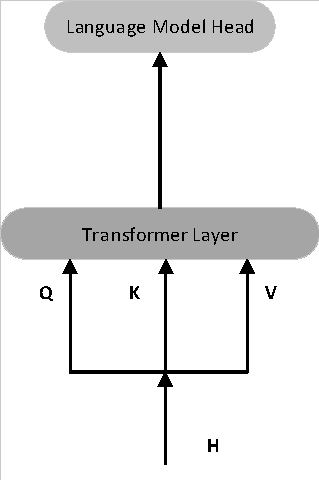
\includegraphics[trim={0.5mm 0.5mm 0.5mm 0.5mm},clip,width=0.35\linewidth]{figures/Model_BERT_S.pdf}
    % \label{fig:bert-a}
}
\hfill
\subfloat[Enhanced Mask Decoder]{
    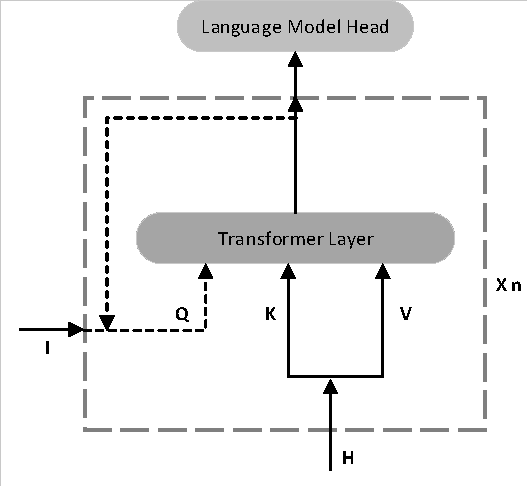
\includegraphics[trim={0.5mm 0.5mm 0.5mm 0.5mm},clip,width=0.58\linewidth]{figures/Model_EMD_S.pdf}
    % \label{fig:emd-b}
}

\caption{BERT 与 DeBERTa 编码层的比较}
\label{fig:emd}
\end{figure*}

将绝对位置信息融入模型有两种方式。BERT模型是在输入层融入绝对位置信息。而在 DeBERTa 结构中,在所有Transformer层之后、但在基于聚合的上下文词内容和位置嵌入来解码掩码词的 Softmax 层之前融入绝对位置信息,如图 \ref{fig:emd} 所示。通过这种方式,DeBERTa 在所有 Transformer 层中捕获相对位置信息,并且仅在解码掩码词时将绝对位置信息作为补充信息使用。因此,DeBERTa 将解码组件称为增强掩码解码器(Enhanced Mask Decoder,EMD)。

\subsubsection{DeBERTa V3 模型}

由于 ELECTRA \cite{clark2020electrapretrainingtextencoders} 中的替换词元检测(Replaced Token Detection, RTD)和 DeBERTa 中的解耦注意力机制已被证明在预训练中样本效率较高,DeBERTa V3 在这两种方法的基础上应运而生。它将原始 DeBERTa 中使用的掩码语言模型(Masked Language Modeling, MLM)目标替换为替换词元检测目标,以结合后者的优势。

基于Transformer的预训练语言模型通常在大量文本上进行预训练,通过一种自监督目标来学习上下文单词表示,这种目标被称为掩码语言建模 \cite{devlin_bert_2019}(MLM)。具体来说,给定一个序列 $X = \{x_i\}$,我们通过随机掩码其15\%的词元将其损坏为 $\tilde{X}$,然后训练一个由 $\theta$ 参数化的语言模型,基于 $\tilde{X}$ 预测被掩码的词元 $\tilde{x}$ 来重建 $X$:
\begin{align}
\max_{\theta} \log p_{\theta}(X|\tilde{X}) = \max_{\theta} \sum_{i \in \mathcal{C}} \log p_{\theta}(\tilde{x}_i = x_i|\tilde{X})
\end{align}
其中,$\mathcal{C}$是序列中被掩码词元的索引集。BERT的作者提议让 10\% 的被掩码词元保持不变,另外 10\% 用随机选择的词元替换,其余的用 [MASK] 词元替换。

与BERT仅使用一个Transformer编码器并通过掩码语言模型进行训练不同,ELECTRA采用生成对抗网络(GAN)的方式,使用两个Transformer编码器进行训练。一个是通过掩码语言模型训练的生成器,另一个是通过词元级二元分类器训练的判别器。生成器用于生成模糊的词元来替换输入序列中被掩码的词元。然后,修改后的输入序列被输入到判别器中。判别器中的二元分类器需要判断相应的词元是原始词元还是由生成器替换的词元。我们分别用 $\theta_G$ 和 $\theta_D$ 表示生成器和判别器的参数。判别器中的训练目标被称为替换词元检测(RTD)。生成器的损失函数可以写为:
\begin{align} 
L_{\text{MLM}} = \mathbb{E} \left( - \sum_{i \in \mathcal{C}} \log p_{\theta_G}(\tilde{x}_{i,G} = x_i|\tilde{\mathbf{X}}_G) \right)
\end{align}
其中,$\tilde{\mathbf{X}}_G$ 是通过在 $\mathbf{X}$ 中随机掩码 15\% 的词元得到的生成器的输入。

判别器的输入序列是通过根据生成器的输出概率采样新的词元来替换被掩码的词元构建的:
\begin{align} 
\tilde{x}_{i,D} = \begin{cases} \tilde{x}_{i} \sim p_{\theta_G}(\tilde{x}_{i,G} = x_i|\tilde{\mathbf{X}}_G), & i \in \mathcal{C} \\ x_i, & i \notin \mathcal{C} \end{cases}
\end{align}

判别器的损失函数可表示为:
\begin{align}
L_{\text{RTD}} = \mathbb{E} \left( - \sum_{i} \log p_{\theta_D} \left( \mathbb{1}(\tilde{x}_{i,D} = x_i)|\tilde{X}_D, i \right) \right) 
\end{align}
其中,$\mathbb{1}(\cdot)$是指示函数,$\tilde{X}_D$是通过公式3构建的判别器的输入。在 ELECTRA 中,$L_{\text{MLM}}$和$L_{\text{RTD}}$是联合优化的,$L = L_{\text{MLM}} + \lambda L_{\text{RTD}}$,其中$\lambda$ 是判别器损失 $L_{\text{RTD}}$ 的权重,在 ELECTRA 中设置为50。 

除此之外,DeBERTa V3 通过用一种新的梯度解耦嵌入共享(Gradient-Disentangled Embedding Sharing, GDES)方法取代 ELECTRA 最初提出的用于替换词元检测的词嵌入共享(Embedding Sharin, ES)方法,使得 DeBERTa V3 的性能得以进一步提升。

\begin{figure*}[htbp]
\centering  
\subfloat[嵌入共享]{
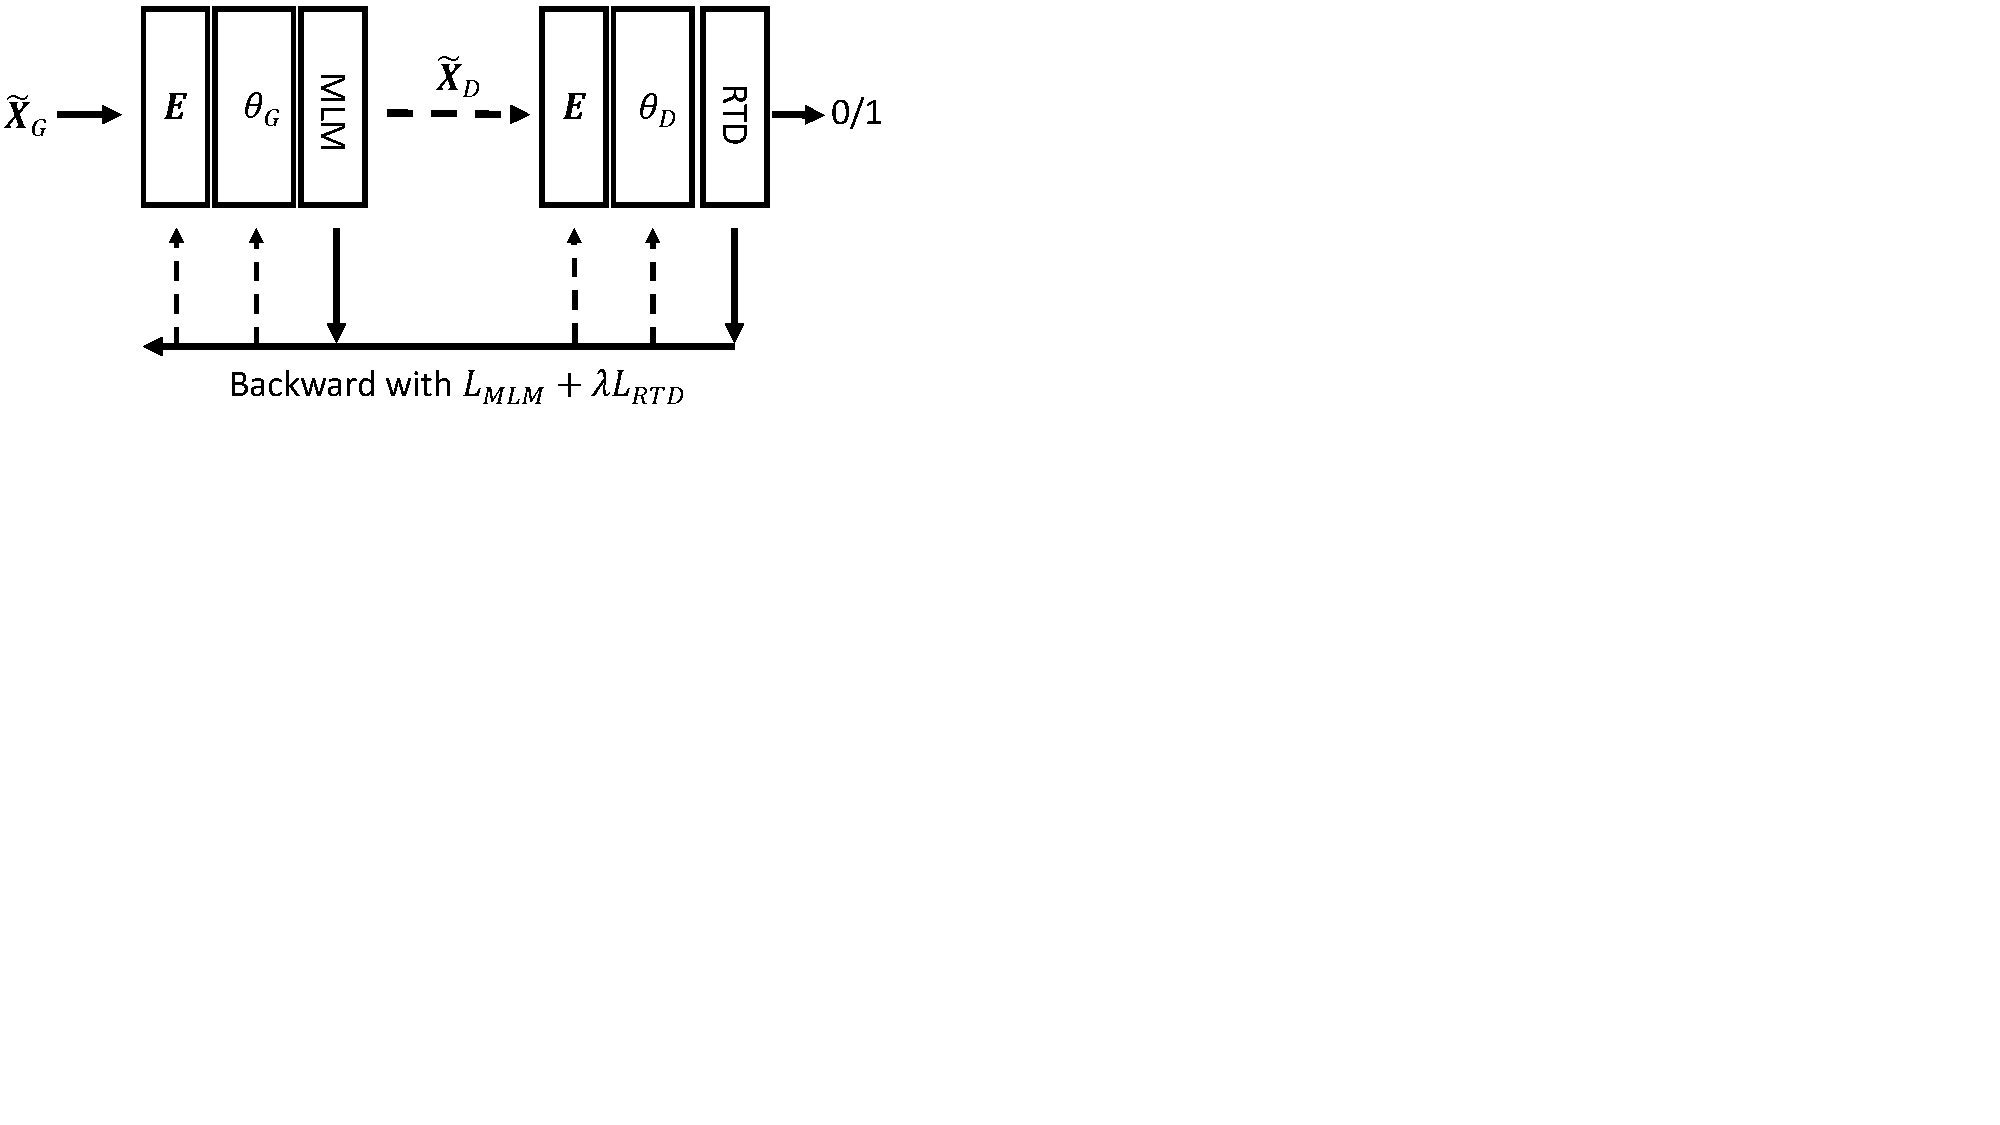
\includegraphics[width=0.31\linewidth,trim={0.1cm 11.8cm 18.5cm 0.1cm},clip]{figures/LRTD-a.pdf}
}
\hfill
\subfloat[无嵌入共享]{
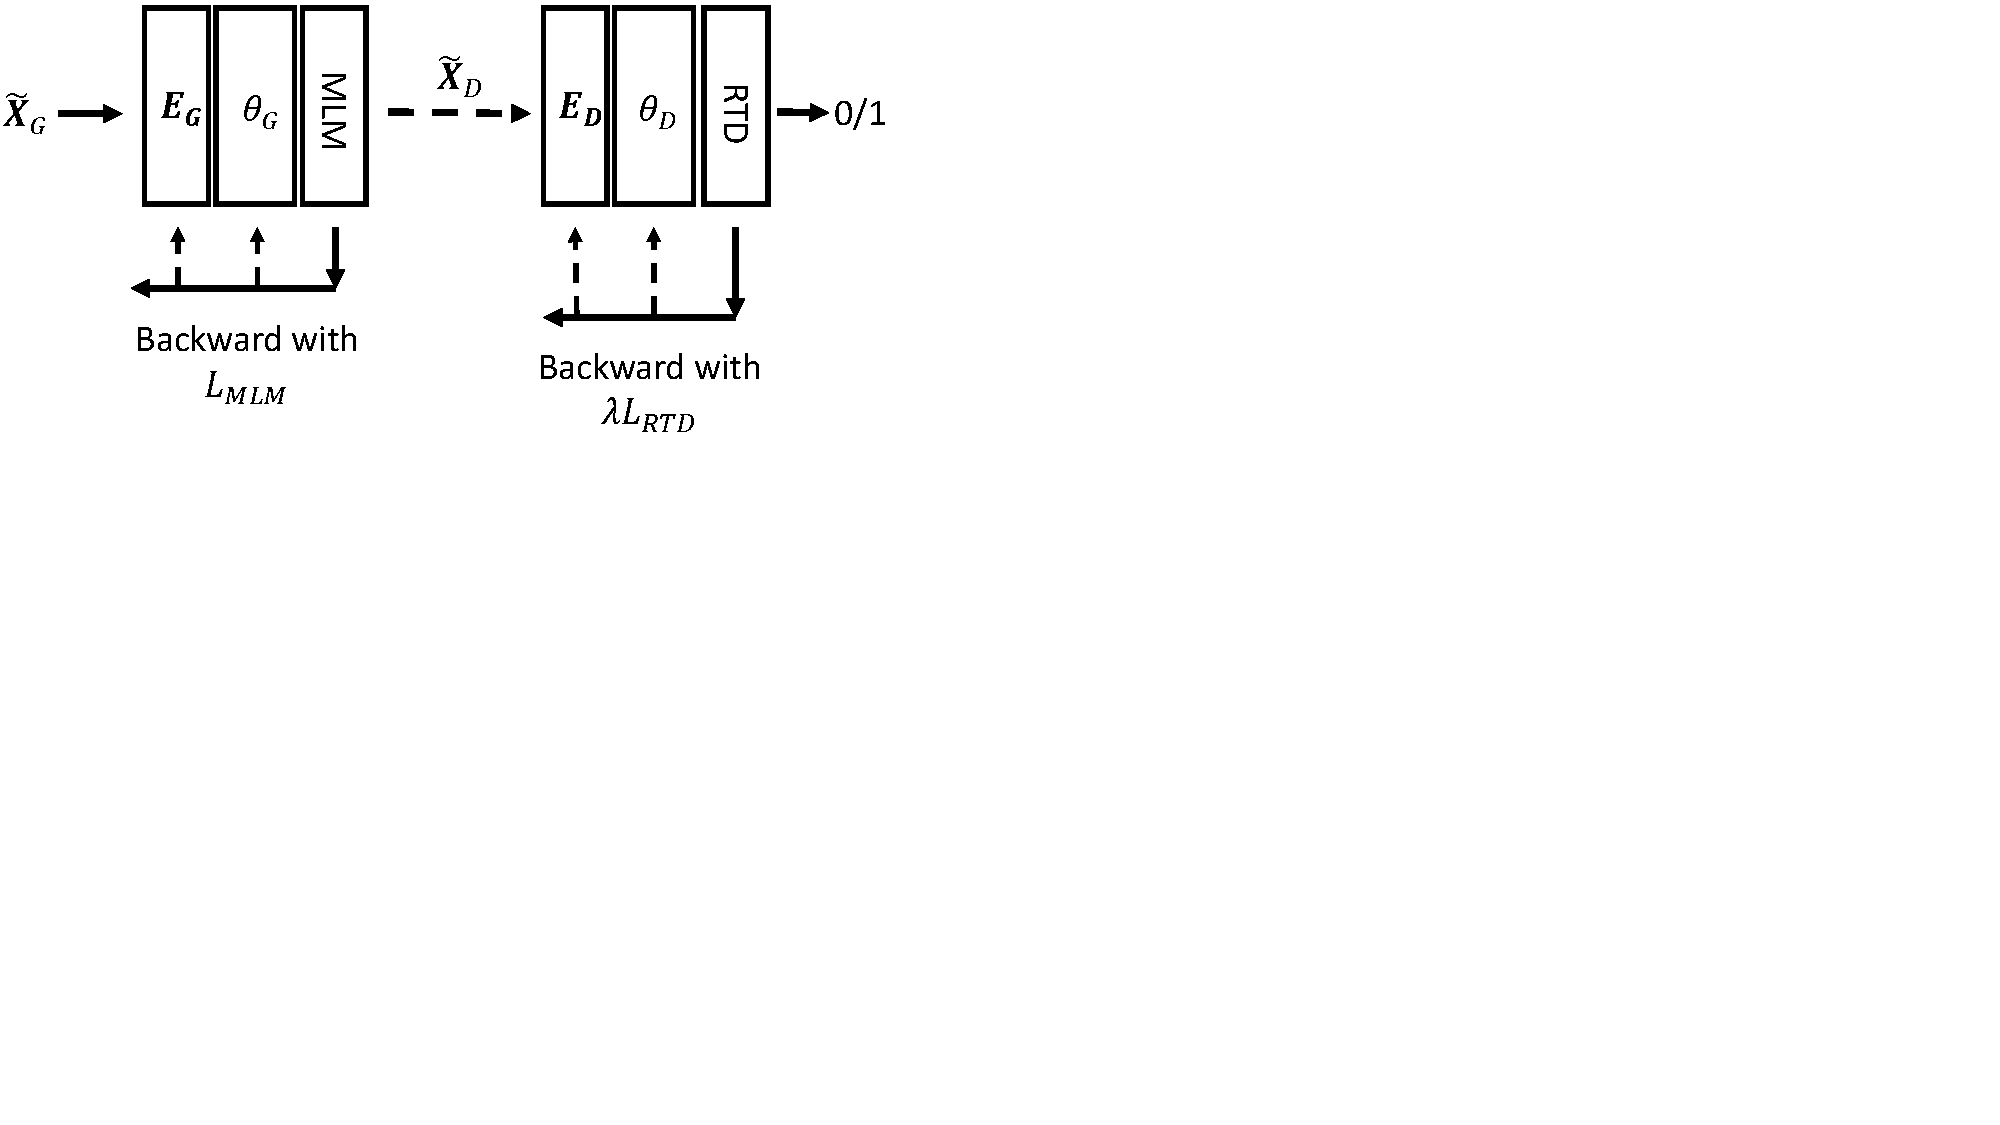
\includegraphics[width=0.31\linewidth,trim={0.1cm 11.7cm 18.5cm 0.1cm},clip]{figures/LRTD-b.pdf}
}
\hfill
\subfloat[梯度解耦嵌入共享]{
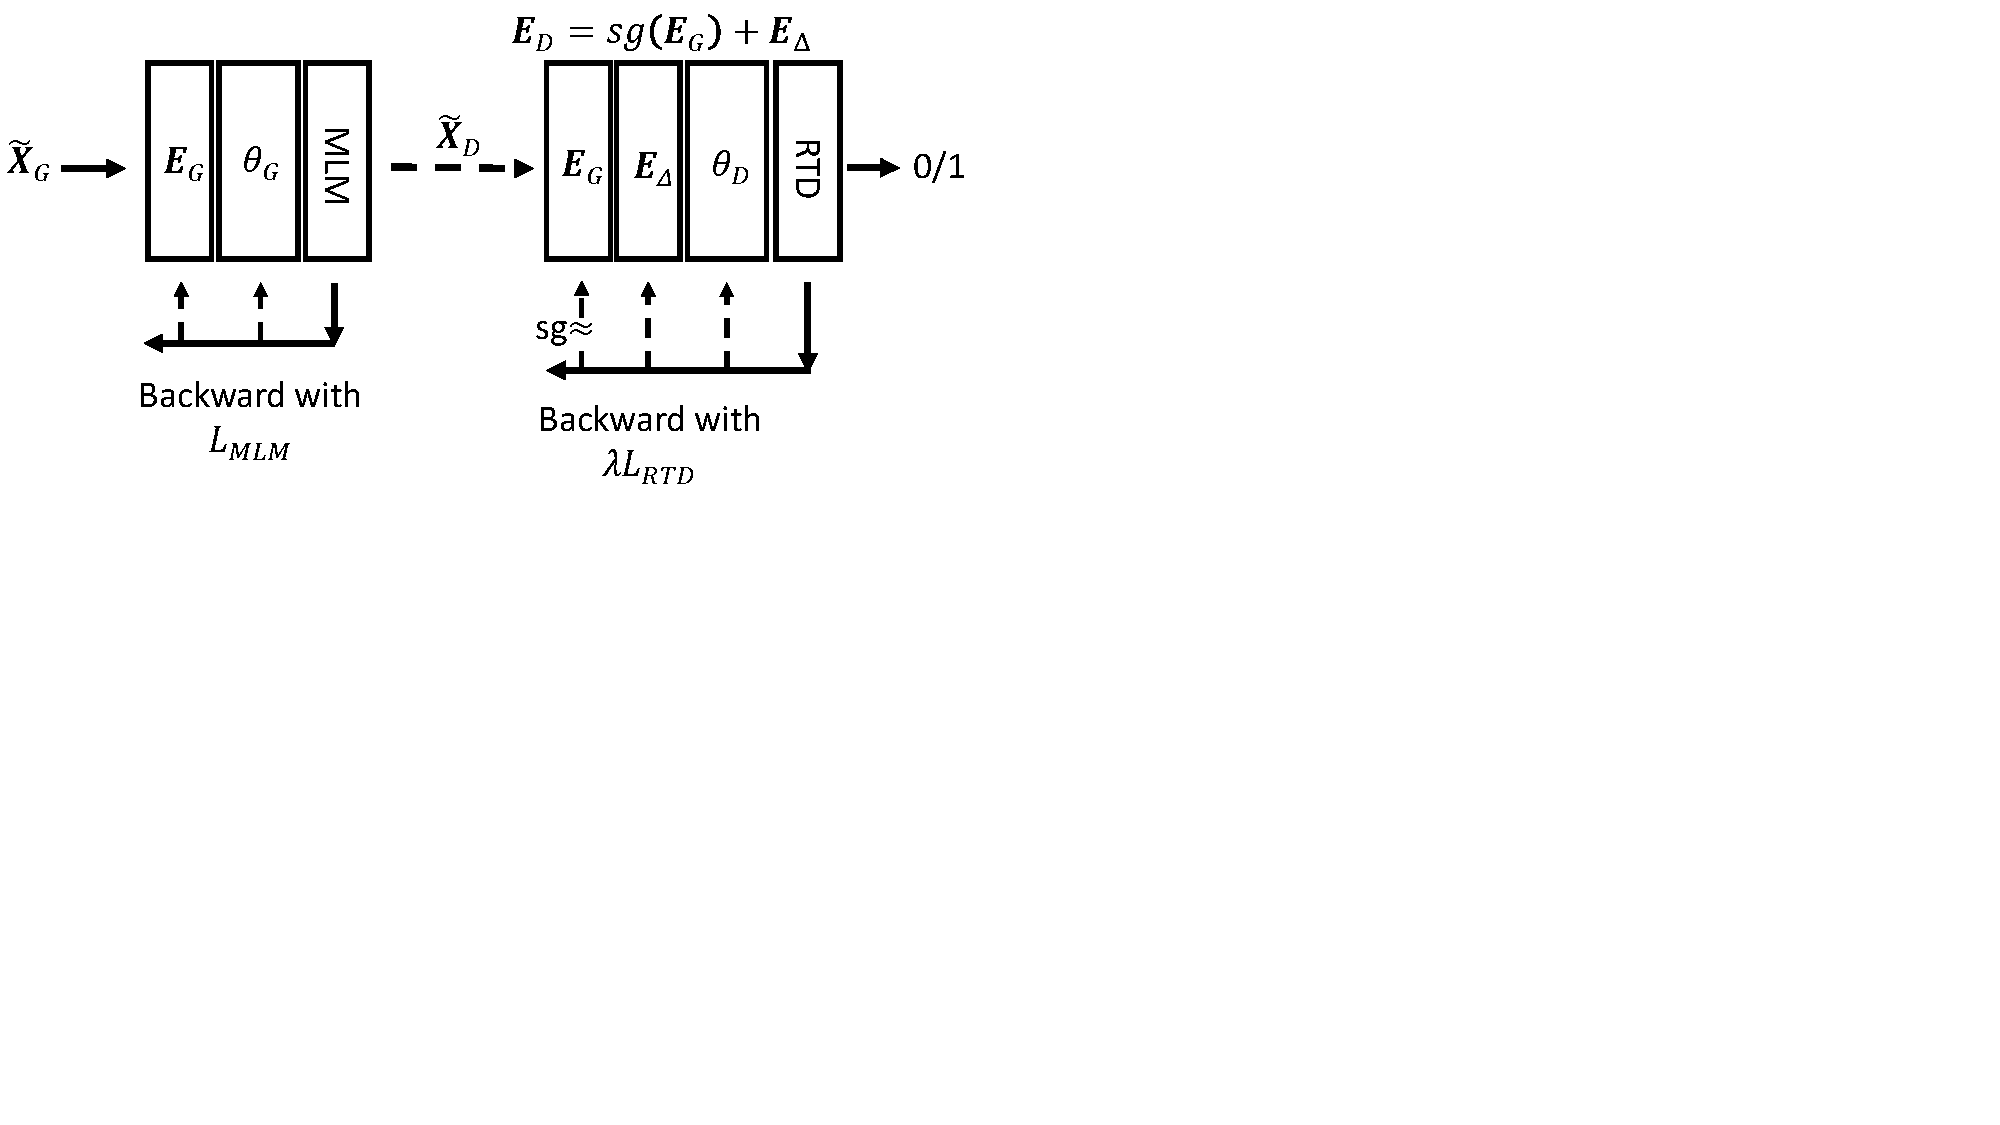
\includegraphics[width=0.31\linewidth,trim={0.1cm 10.4cm 17.5cm 0.1cm},clip]{figures/LRTD-c.pdf}
}
\caption{不同嵌入共享方法示意图}
\label{fig:es}
\end{figure*}

DeBERTa V3 提出梯度解耦嵌入共享(Gradient-Disentangled Embedding Sharing, GDES)方法,以克服嵌入共享(Embedding Sharin, ES)和无嵌入共享(No Embedding Sharin, NES)的缺点,同时保留它们的优点。图 \ref{fig:es} 中展示了不同嵌入共享方法示意图。嵌入共享(Embedding Sharin, ES)中,$\mathbf{E}$、$\theta _ G$ 和 $\theta _ D$ 将在一次反向传播中依据 $L _ {\text{MLM}} + \lambda L _ {\text{RTD}}$ 共同更新。无嵌入共享(No Embedding Sharin, NES)中,$\mathbf{E}_{G}$ 和 $\theta _ G$ 将首先依据 $L_{\text{MLM}}$ 通过反向传播进行更新,然后 $\mathbf E_{D}$ 和 $\theta _ D$ 将依据 $\lambda L _ {RTD}$ 通过反向传播进行更新。而在梯度解耦嵌入共享(Gradient-Disentangled Embedding Sharing, GDES)中,$\mathbf E _ {G}$ 和 $\theta _ G$ 将首先依据 $L_{\text{MLM}}$ 在反向传播中进行更新,然后 $\mathbf E_{\Delta}$ 和 $\theta _ D$ 将依据 $\lambda L _ {\text{RTD}}$ 和 $\mathbf E_{G}$ 通过反向传播进行更新。 $sg$ 是停止梯度操作符,用于防止判别器更新 $\mathbf E _ G$。

如图 \ref{fig:es}(c)所示,梯度解耦嵌入共享方法在生成器和判别器之间共享词嵌入,这使得两个模型能够从相同的词汇表中学习,并利用嵌入中编码的丰富语义信息。然而,与嵌入共享方法不同,梯度解耦嵌入共享方法不允许替换词元检测损失影响生成器的梯度,从而避免了由冲突目标导致的干扰和效率低下问题。相反,梯度解耦嵌入共享方法仅使用掩码语言模型损失来更新生成器的嵌入,这确保了生成器输出的一致性和连贯性。结果,梯度解耦嵌入共享方法可以达到与无嵌入共享相同的收敛速度,同时又不牺牲嵌入的质量。

为了实现梯度解耦嵌入共享,DeBERTa V3 将判别器的嵌入重新参数化为 $\mathbf{E}_D = sg(\mathbf{E}_G) + \mathbf E_{\Delta}$,其中停止梯度算子 $sg$ 可防止梯度流经生成器的嵌入$\mathbf E_G$,仅更新残差嵌入$\mathbf E_{\Delta}$。DeBERTa V3 将$\mathbf E_{\Delta}$初始化为零矩阵,并按照无嵌入共享的训练过程进行模型训练。在每次迭代中,首先使用生成器为判别器生成输入,并利用掩码语言模型损失更新$\mathbf E_G$和$\mathbf E_D$。然后,在生成的输入上运行判别器,并利用梯度解耦嵌入共享损失更新 $\mathbf E_D$,但仅通过 $\mathbf E_{\Delta}$ 进行更新。训练完成后,将 $\mathbf E_{\Delta}$ 加到 $\mathbf E_G$ 上,并将得到的矩阵保存为判别器的 $\mathbf E_D$。

DeBERTa V3 进行了广泛的实验,以评估梯度解耦嵌入共享与嵌入共享和无嵌入共享相比的有效性。其结果证实,梯度解耦嵌入共享是一种用于使用掩码语言模型和替换词元检测进行预训练的语言模型的有效权重共享方法。也因此,DeBERTa V3 模型成为了目前 Kaggle 刷榜以及深度学习效果相当强大的模型。我们在本实验中使用的 DeBERTa 系列模型包括 DeBERTa-V3-Base 和 DeBERTa-V3-Large,表 \ref{tab:deberta-parameter} 中展示了其模型参数。

\begin{table*}[htbp]
\centering
\caption{DeBERTa-V3-Base 和 DeBERTa-V3-Large 模型参数} \label{tab:deberta-parameter}
\begin{tabular}{lcc}
\toprule
               & \multicolumn{1}{l}{\textbf{DeBERTa-V3-Base}} & \multicolumn{1}{l}{\textbf{DeBERTa-V3-Large}} \\ \midrule
Transformer 层数 & 12                                           & 24                                            \\
隐藏层维度          & 768                                          & 1024                                          \\
词汇表大小          & 128K                                         & 128K                                          \\
主干网络参数量        & 86M                                          & 304M                                          \\
嵌入层参数量         & 98M                                          & 131M                                \\ \bottomrule         
\end{tabular}
\end{table*}

\section{实验设计}
\label{sec:method-experiment}

我们设计了如下实验,基于在第 \ref{chap:TOSWT} 章中介绍的模型改写文本检测数据集微调 \ref{sec:method-pretrain-roberta} 节中提及的 RoBERTa-Base 和 RoBERTa-Large 以及在 \ref{sec:method-pretrain-deberta} 节中提及的 DeBERTa-V3-Base 和 DeBERTa-V3-Large 模型。微调后再调用模型在测试集上输出预测标签,最后使用四种指标准确率(Accuracy)、精确率(Precision)、召回率(Recall)和 F1 分数评估预测标签的水准,进而评定微调后的模型能力。

为满足细粒度的数据要求,分别使用文档级别和句子级别的数据分别微调上文提及的四个模型。这些预训练模型参数来源 URL 如表 \ref{tab:method-pretrain_model_url} 所示。

\begin{table*}[htbp]
\centering
\caption{预训练模型参数来源 URL} \label{tab:method-pretrain_model_url}
\begin{tabular}{ll}
\toprule
\textbf{模型}      & \textbf{URL}                                                                 \\ \midrule
RoBERTa-Base     & https://huggingface.co/FacebookAI/roberta-base    \\
RoBERTa-Large    & https://huggingface.co/FacebookAI/roberta-large   \\
DeBERTa-V3-Base  & https://huggingface.co/microsoft/deberta-v3-base  \\
DeBERTa-V3-Large & https://huggingface.co/microsoft/deberta-v3-large \\ \bottomrule
\end{tabular}
\end{table*}

除了该对比实验外,我们还设计了消融实验,在 AES2 数据集评分基础上,进一步探索大语言模型改写文本的能力。有这样两个问题:原始文本对于大语言模型改写文本的影响有多大?大语言模型改写文本后,新文本的文本质量与原始文本质量一致性如何?为深入探索这两个问题,我们同样设计了两个额外的消融实验放置于 \ref{sec:method-experiment-analysis} 中。

\subsection{数据集设置}
\label{sec:method-experiment-dataset}

本实验中数据集采用在第 \ref{chap:TOSWT} 章中介绍的模型改写文本检测数据集。数据集示例如表 \ref{tab:TOSWT-eg} 所示,受单页篇幅所限,这里选取了一个包含两个句子的数据示例,该示例数据评分在其原始 AES2 数据集中被评定为 2 分。

\begin{table*}[htbp]
\BITSetup{ misc / tabularFontSize = 6}
\centering
\caption{模型改写文本检测数据集数据示例} \label{tab:TOSWT-eg}
\begin{tabular}{lp{12cm}}
\toprule
\multicolumn{1}{c}{\textbf{模型}} & \multicolumn{1}{c}{\textbf{文本}}  \\ \midrule
AES2                            & Luke think you should join the   seagoing cowboys program because you can travel all around and see some   pretty nice things like Luke it said in the passage that you take nine trips   to things like Greece,China,you will past the Atlantic Ocean and also you can   make the world a better place and you can be a hero for being nice. Also so if you want to you can help out animals in the passage it said, the   animals had to drink two or three times a day also a way you can help you   could clean the stalls on the ship and they will give you jobs and other   stuff and so you won't think it is boring you can have fun onboard to they   got a lot of things like baseball,and volleyball and the house it is   table-tennis tournaments,fencing,boxing,reading,whittling,and the games make   time go fast and that's why I think you should join the seagoing Cowboys   program. \\ \midrule
GPT3.5                          & Luke thinks you should   join the Seagoing Cowboys program because you can travel all around and see   some pretty nice things. Like Luke said in the passage, you can take nine   trips to places like Greece and China. You will cross the Atlantic Ocean, and   you can make the world a better place by being nice and becoming a   hero. Also, if you want to, you can help out animals. In the passage, it said   that the animals had to drink two or three times a day. Another way you can   help is by cleaning the stalls on the ship. They will give you jobs and other   stuff. And so you won't think it's boring, you can have fun onboard too. They   have a lot of things like baseball, volleyball, table-tennis tournaments,   fencing, boxing, reading, and whittling. The games make time go fast, and   that's why I think you should join the Seagoing Cowboys program.   \\ \midrule
GPT4o                           & Luke believes you should join the seagoing   cowboys program because it allows you to travel extensively and see beautiful   places; as mentioned in the passage, you can undertake trips to destinations   like Greece and China, cross the Atlantic Ocean, and make the world a better   place while becoming a hero by being kind. Additionally, if you wish, you can assist with caring for animals; the   passage noted that the animals need to drink two or three times a day, and   one of the ways you can contribute is by cleaning the stalls on the ship,   where they will provide you with various tasks to keep you engaged, along   with fun activities such as baseball and volleyball, as well as other   pastimes like table tennis tournaments, fencing, boxing, reading, whittling,   which help make the time fly by-these are the reasons I think you should join   the seagoing Cowboys program. \\ \midrule
Gemini                          & Luke believes you should join   the Seagoing Cowboys program because it offers the opportunity to travel   extensively and witness beautiful sights, as he mentioned in the passage that   participants take nine trips to destinations like Greece and China, traverse   the Atlantic Ocean, and contribute to making the world a better place,   potentially becoming a hero through acts of kindness. Additionally, if you're interested, you can assist animals, as the passage   mentioned that they need to drink two or three times daily; you could also   help by cleaning stalls on the ship, and they'll provide you with various   tasks and activities to keep you engaged and prevent boredom, as there are   plenty of recreational options onboard, including baseball, volleyball, table   tennis tournaments, fencing, boxing, reading, whittling, all of which help   pass the time quickly, and that's why I believe you should consider joining   the Seagoing Cowboys program. \\ \midrule
Qwen                            & Luke believes you should join   the seagoing cowboys program because it offers opportunities to travel   extensively and see beautiful places, such as Greece and China, as mentioned   in the passage. You will cross the Atlantic Ocean and contribute to making the   world a better place, thereby becoming a hero by being kind and   helpful. Additionally, if you wish, you can assist animals, as the passage notes   they need to drink two or three times a day. You could help by cleaning the   ship's stalls and taking on various jobs, ensuring the journey is enjoyable.   Onboard activities like baseball, volleyball, table tennis tournaments,   fencing, boxing, reading, and whittling make time pass quickly, which is why   I think you should join the seagoing cowboys program. \\ \midrule
DeepSeek                        & Luke believes you should join   the seagoing cowboys program because it offers the opportunity to travel   extensively and witness beautiful sights, such as Greece and China, while   crossing the Atlantic Ocean, and it allows you to make the world a better place   and become a hero through kindness. Additionally, if you wish, you can assist animals, as mentioned in the   passage, which require drinking two or three times daily, and you can   contribute by cleaning the stalls on the ship, where they provide jobs and   other activities to ensure it's not boring; you can also enjoy onboard   entertainment like baseball, volleyball, table-tennis tournaments, fencing,   boxing, reading, whittling, and games that make time pass quickly, which is   why I recommend joining the seagoing cowboys program. \\ \bottomrule
\end{tabular}
\end{table*}

对于文档级数据,我们将模型改写文本检测数据集分割为训练集、验证集与测试集。这三个被分割后的小数据集在大数据集随机打乱后分别按照文档的个数以 $7:1:2$ 的比例分割出来。待微调的模型在训练集上微调过后,该模型在验证集上得到初步的模型效果,随后选取损失函数最低的模型在测试集上测试,进而得到最终的效果。

而句子级数据中关于数据集的分割步骤也与文档级数据的分割步骤类似。只不过第一步需要先将所有句子分割出来,单独打上标签,按照句子的个数随机打乱顺序后再以 $7:1:2$ 的比例分割为训练集、验证集和测试集。

对于词元个数过长的数据用例,我们将长度大于 512 后面的部分完全截断。不过,这一步是在词元化(tokenizer)的过程中处理的。

\subsection{实验参数设置}
\label{sec:method-experiment-parameter}

所有实验均运行于 Ubuntu Linux 22.04 服务器上。详细实验操作系统环境如表 \ref{tab:os-env} 所示。

\begin{table*}[htbp]
\centering
\caption{实验操作系统环境} \label{tab:os-env}
\begin{tabular}{ll}
\toprule
\textbf{字段}    & \textbf{值}                               \\ \midrule
内核版本           & 6.8.0-49-generic                         \\
构建环境           & buildd@lcy02-amd64-103                   \\
架构             & x86\_64 (64位)                             \\
编译器            & x86\_64-linux-gnu-gcc-12                  \\
编译器版本          & 12.3.0                                   \\
编译器来源          & Ubuntu 12.3.0-1ubuntu1\textasciitilde22.04             \\
链接器   (GNU ld) & GNU Binutils for Ubuntu 2.38             \\
构建编号           & \#49\textasciitilde22.04.1-Ubuntu                       \\
构建类型           & SMP (对称多处理) + PREEMPT\_DYNAMIC(动态抢占模式) \\
构建时间           & Wed Nov 6 17:42:15 UTC 2024              \\
发行版基础          & Ubuntu 22.04.1 LTS                       \\ \bottomrule
\end{tabular}
\end{table*}

本章节全部实验均在拥有 24GB 显存容量的 NVIDIA TITAN RTX 显卡上完成,该显卡详细环境如表 \ref{tab:gpu-env} 所示。

\begin{table*}[htbp]
\centering
\caption{实验显卡环境} \label{tab:gpu-env}
\begin{tabular}{ll}
\toprule
\textbf{字段} & \textbf{值}           \\ \midrule
GPU   型号    & NVIDIA TITAN RTX     \\
GPU   架构    & Turning              \\
显存容量        & 24GB                 \\
TDP   (功耗)  & 320W                 \\
驱动版本        & NVIDIA-SMI 560.35.03 \\
CUDA   版本   & 12.6                 \\ \bottomrule
\end{tabular}
\end{table*}

本章节实验在实现上基于 Anaconda 库中搭建的 Conda 虚拟环境运行 Python 代码,Python 环境中部分重要包版本号如表 \ref{tab:python-env} 所示。

\begin{table*}[htbp]
\BITSetup{ misc / tabularFontSize = 6}
\centering
\caption{实验 Python 环境部分重要包版本} \label{tab:python-env}
\begin{tabular}{cll}
\toprule
\textbf{分类}                  & \textbf{字段}       & \textbf{版本号} \\ \midrule
\multirow{28}{*}{基础}         & conda             & 24.9.2       \\
                             & Python            & 3.12.8       \\
                             & GCC               & 11.2.0       \\
                             & cuda-cudart       & 11.8.89      \\
                             & cuda-cupti        & 11.8.87      \\
                             & cuda-libraries    & 11.8.0       \\
                             & cuda-nvrtc        & 11.8.89      \\
                             & cuda-nvtx         & 11.8.86      \\
                             & cuda-runtime      & 11.8.0       \\
                             & cuda-version      & 12.6         \\
                             & ipython           & 8.30.0       \\
                             & json5             & 0.9.25       \\
                             & matplotlib        & 3.9.2        \\
                             & matplotlib-base   & 3.9.2        \\
                             & matplotlib-inline & 0.1.6        \\
                             & nltk              & 3.9.1        \\
                             & numpy             & 2.0.1        \\
                             & openai            & 1.52.1       \\
                             & pandas            & 2.2.3        \\
                             & pillow            & 11.0.0       \\
                             & pip               & 24.2         \\
                             & regex             & 2024.11.6    \\
                             & sentencepiece     & 0.2.0        \\
                             & scikit-learn      & 1.6.0        \\
                             & scipy             & 1.14.1       \\
                             & tensorboard       & 2.17.0       \\
                             & xlsxwriter        & 3.1.1        \\
                             & yaml              & 0.2.5        \\ \midrule
\multirow{6}{*}{Torch}       & pytorch           & 2.5.1        \\
                             & pytorch-cuda      & 11.8         \\
                             & pytorch-mutex     & 1.0          \\
                             & torchaudio        & 2.5.1        \\
                             & torchtriton       & 3.1.0        \\
                             & torchvision       & 0.20.1       \\ \midrule
\multirow{5}{*}{HuggingFace} & accelerate        & 1.2.1        \\
                             & datasets          & 3.2.0        \\
                             & huggingface-hub   & 0.27.0       \\
                             & tokenizers        & 0.21.0       \\
                             & transformers      & 4.47.1       \\ \bottomrule
\end{tabular}
\end{table*}

在基础的文档级和句子级的数据实验中,我们使用 DeBERTa 和 RoBERTa 作为实验用的模型并微调了四种模型:RoBERTa-Base、RoBERTa-Large、DeBERTa-Base 和 DeBERTa-Large,可变超参数包括批大小(batch size, BS)、学习率(learning rate, LR)、权重衰减系数(weight decay, WD)。在所有实验中,学习率均采用余弦退火衰减算法,并使用 AdamW 算法作为优化器。超参数详见表 \ref{tab:hyper-parameters},其中,在句子级实验中,大尺寸模型如 RoBERTa-Large 和 DeBERTa-V3-Large 的超参数均经过广泛地搜索长时间实验才找到可以使模型拟合于数据的一组超参数。DeBERTa-V3-Large 由于其总参数量较大,为防止超出显卡显存,因此批大小相较其他实验的 16 个为一批较小,设置为 4 个为一批。

\begin{table*}[htbp]
\centering
\caption{对比试验微调超参数列表}
\label{tab:hyper-parameters}
\begin{tabular}{c|l|ccc}
\toprule
                          & \textbf{模型}   & \textbf{批大小} & \textbf{初始学习率} & \textbf{权重衰减系数} \\ \midrule
\multirow{4}{*}{文档级}    & RoBERTa-Base     & 16                  & $10^{-5}$                & 0.01                  \\
                          & RoBERTa-Large    & 16                  & $10^{-5}$                & 0.01                  \\
                          & DeBERTa-V3-Base  & 16                  & $10^{-5}$                & 0.01                  \\
                          & DeBERTa-V3-Large & 4                   & $10^{-5}$                & 0.01                  \\ \midrule
\multirow{4}{*}{句子级}    & RoBERTa-Base     & 16                  & $10^{-5}$                & 0.01                  \\
                          & RoBERTa-Large    & 16                  & $10^{-6}$               & 0.0001                \\
                          & DeBERTa-V3-Base  & 16                  & $10^{-5}$                & 0.01                  \\
                          & DeBERTa-V3-Large & 4                   & $10^{-6}$               & 0.001                 \\ \bottomrule
\end{tabular}
\end{table*}

\subsubsection{交叉熵损失函数}

交叉熵函数 \cite{CrossEntropy} 是信息论和机器学习中的核心概念,主要用于衡量两个概率分布之间的差异。其数学定义为:对于真实分布 $P$ 和预测分布 $Q$,交叉熵 $H(P,Q)=-\sum_x P(x)\log Q(x)$。它表示用 $Q$ 编码来自 $P$ 的事件所需的平均比特数,当 $Q$ 越接近 $P$ 时,交叉熵值越小。

在机器学习中,交叉熵常作为分类任务的损失函数。例如,在本文中,对于 $m$ 个样本的 $6$ 分类问题,损失函数可表示为 
\begin{align}
L=-\frac{1}{m}\sum_{i=1}^m \sum_{j=1}^6 t_{ij}\log(y_{ij})
\end{align}
其中 $t_{ij}$ 是真实标签(one-hot编码),$y_{ij}$ 是模型预测概率。这种设计能有效惩罚预测错误,尤其配合 Softmax 或 Sigmoid 激活函数时,梯度计算高效且避免均方误差的学习速率下降问题。

交叉熵与信息熵、KL散度密切相关。信息熵 $H(P)$ 是 $P$ 自身的最佳编码长度,而交叉熵 $H(P,Q)$ 是使用 $Q$ 编码 $P$ 的代价,两者差值即为 KL 散度,反映分布差异。实际应用中需注意数值稳定性,如对 $Q(x)$ 裁剪防止 $\log(0)$ 错误。

将交叉熵函数作为损失函数,其优势在于理论严谨性与实践高效性的结合。例如,图像分类任务中,交叉熵直接优化预测概率与真实标签的匹配度;在本文所处的领域自然语言处理中,它评估生成文本的概率分布质量。

\subsubsection{AdamW 优化器}

AdamW 优化器 \cite{AdamW} 是 Adam 优化器 \cite{Adam} 的一个改进版本,算法流程如算法 \ref{algo:AdamW} 所示。Ilya Loshchilov 和 Frank Hutter 在 2017 年提出该算法,主要解决了传统 Adam 优化器中权重衰减(Weight Decay)处理方式的问题。在原始的 Adam 优化器中,权重衰减是通过将衰减项直接添加到梯度中来实现的,这种方式会导致权重衰减的效果受到自适应学习率的干扰,从而影响正则化的有效性。而 AdamW 通过将权重衰减从梯度更新过程中解耦,使其直接作用于参数更新步骤,从而更准确地实现正则化效果。

\begin{algorithm}[htb]
\caption{AdamW 优化算法} \label{algo:AdamW}
\begin{algorithmic}[1]
    \Require 学习率 $\psi(\text{lr})$, $\beta_1$, $\beta_2$ (betas), 初始参数 $\theta_0$ (params), 目标函数 $f(\theta)$ (objective), $\epsilon$, 权重衰减 $\chi$, amsgrad, maximize
    \Ensure $\theta_t$
    
    \State 初始化: $m_0 \leftarrow 0$ (一阶矩), $v_0 \leftarrow 0$ (二阶矩), $\widehat{v_0}^{max} \leftarrow 0$
    \For {$t = 1$ to $\ldots$}
        \If{maximize}
            \State $g_t \leftarrow - \nabla_\theta f_t(\theta_{t-1})$
        \Else
            \State $g_t \leftarrow \nabla_\theta f_t(\theta_{t-1})$
        \EndIf
        
        \State $\theta_t \leftarrow \theta_{t-1} - \psi \chi \theta_{t-1}$ \Comment{权重衰减}
        
        \State $m_t \leftarrow \beta_1 m_{t-1} + (1 - \beta_1) g_t$ \Comment{更新一阶矩}
        \State $v_t \leftarrow \beta_2 v_{t-1} + (1 - \beta_2) g_t^2$ \Comment{更新二阶矩}
        
        \State $\widehat{m_t} \leftarrow m_t / (1 - \beta_1^t)$ \Comment{偏差修正}
        \State $\widehat{v_t} \leftarrow v_t / (1 - \beta_2^t)$
        
        \If{amsgrad}
            \State $\widehat{v_t}^{max} \leftarrow \max(\widehat{v_{t-1}}^{\text{max}}, \widehat{v_t})$
            \State $\theta_t \leftarrow \theta_t - \psi \widehat{m}_t / (\sqrt{\widehat{v_t}^{\text{max}}} + \epsilon)$
        \Else
            \State $\theta_t \leftarrow \theta_t - \psi \widehat{m_t} / (\sqrt{\widehat{v_t}} + \epsilon)$
        \EndIf
    \EndFor
\end{algorithmic}
\end{algorithm}

AdamW 的核心思想是保留 Adam 优化器的自适应学习率和动量机制,同时改进权重衰减的处理方式。具体来说,AdamW 在参数更新时,将权重衰减项独立于梯度计算之外,直接对参数进行衰减。这种方法使得权重衰减的效果更加稳定,能够有效防止模型过拟合,并提升泛化能力。实验表明,AdamW 在多个深度学习任务中表现优于传统的 Adam,尤其是在需要强正则化的场景下。

AdamW 的优点包括:1) 更有效的正则化,能够更好地控制模型复杂度;2) 在训练深度神经网络时表现出更稳定的收敛性;3) 适用于需要长时间训练的任务,如大语言模型(LLM)的预训练。然而,AdamW 也有一些缺点,例如对学习率和权重衰减系数的选择较为敏感,需要更多的调参工作,这也导致了句子级尺寸较大的模型调参工作较为繁琐。

在实际应用中,AdamW 已成为许多深度学习框架(如 PyTorch)的默认优化器之一,特别适合处理高维参数空间和复杂模型结构。它的改进设计使其在保持 Adam 高效性的同时,进一步提升了模型的泛化性能,成为现代深度学习训练中的重要工具。

\subsubsection{余弦退火调度器}

余弦退火是一种在深度学习中广泛使用的学习率调度策略,其核心思想是通过余弦函数动态调整学习率,以优化模型训练过程。该方法最初由 Ilya Loshchilov 和 Frank Hutter 在2016年的 SGDR 方法 \cite{SGDR} 中提出,随后成为深度学习领域的重要技术。余弦退火的名称来源于其数学实现方式——学习率按照余弦函数曲线从初始值平滑下降到最小值,类似于金属加工中的退火过程,即先高温加热后缓慢冷却。

从数学原理来看,余弦退火的公式为
\begin{align}
\eta_t = \eta_{min} + \frac{1}{2}(\eta_{max} - \eta_{min})(1 + \cos(\frac{T_{cur}}{T_i}\pi))
\end{align}
其中$\eta_{max}$和$\eta_{min}$分别表示学习率的上下界,$T_{cur}$是当前训练步数,$T_i$是总步数。这种设计使得学习率在训练初期保持较大值以加速收敛,随后逐渐减小以便模型精细调整参数。与传统的阶梯式衰减或线性衰减相比,余弦退火提供了更平滑的过渡,避免了学习率突变导致的训练不稳定。

在实际应用中,余弦退火具有多重优势。首先,其周期性调整特性有助于模型跳出局部最优解,这在处理多峰损失函数时尤为有效。其次,该方法减少了人工调参需求,通过预设的数学规律自动调整学习率,适用于各种复杂模型和大规模数据集。实验表明,在图像分类、自然语言处理等任务中,采用余弦退火策略的模型通常能获得更快收敛速度和更好泛化性能。例如在ImageNet竞赛中,ResNet模型采用该策略后表现出显著提升。

\subsubsection{权重衰减算法}

权重衰减是深度学习中一种常用的正则化技术,主要用于防止模型过拟合。其核心原理是通过在损失函数中添加与权重参数平方和成正比的惩罚项(即$L_2$范数),约束模型参数的幅度。具体公式为
\begin{align}
L' = L + \lambda \sum \theta_i^2
\end{align}
其中$L$是原始损失函数,$\theta$ 为模型权重,$\lambda$为正则化系数,控制惩罚强度。这种设计迫使模型在训练过程中倾向于学习较小的权重值,从而降低模型复杂度,避免对训练数据中的噪声过度敏感。

从实现机制来看,权重衰减在梯度下降过程中会直接影响参数更新。以随机梯度下降为例,这种操作相当于在每次迭代时对权重施加线性衰减,因此得名"权重衰减"。值得注意的是,权重衰减通常不应用于偏置项,因为偏置主要控制输出平移,对模型复杂度影响较小。

权重衰减的作用机理可从多角度解释。首先,较小的权重使模型对输入变化更鲁棒,减少对噪声特征的依赖;其次,通过抑制特征间的共线性,避免模型过度依赖某些特定特征组合;最后,它能有效防止梯度爆炸问题,提升训练稳定性。实验表明,在ImageNet等大型数据集上,合理设置$\lambda$可使测试误差降低10\%-20\%。

实际应用中,权重衰减常与其他技术(如Dropout、批量归一化)结合使用。超参数$\lambda$的选择需通过多次验证确定,典型取值范围为$10^{-4}$到$10^{-2}$,在本文中经多次测试找出相应权重衰减超参数。现代深度学习框架如本文使用的 PyTorch 中内置了权重衰减功能,通过上文提及的 AdamW 优化器的 weight\_decay 参数即可启用。需要注意的是,权重衰减与$L_2$正则化数学形式相似,但实现机制存在差异:前者直接修改优化过程,后者通过损失函数间接作用。

\subsection{评价指标}
\label{sec:method-experiment-metric}

本文共使用四种评价指标来评定,分别为\textbf{准确率}(Accuracy)、\textbf{精准率}(Precision)、\textbf{召回率}(Recall)和 \textbf{F1 分数}。这四种评价指标将在下面的小节中进行相应的介绍。由于模型改写文本检测本质上是多分类文本分类任务,因此后三者指标需要与二分类指标有相应变化。由于每个生成模型产生相同数量的文本,并且由于数据量对指标的影响最小,因此采用了对数据量敏感的宏观(macro)方法。

以及会介绍一下在后面的章节 \ref{sec:method-experiment-analysis} 中涉及到的 spearman 系数和 pearson 系数。此二者系数用于衡量生成的文本评估的分数与原始 AES2 数据集中数据分数的相关性与一致性。

\subsubsection{准确率}

准确率(Accuracy)是机器学习中最基础且直观的分类评估指标,用于衡量模型整体预测的正确性。其核心定义为模型正确预测的样本数占总样本数的比例,数学表达式为 
\begin{align}
    Accuracy = \frac{TP+TN}{TP+TN+FP+FN}
\end{align}
其中 $TP$(真正例)和 $TN$(真负例)分别表示正负类预测正确的数量,$FP$(假正例)和 $FN$(假负例)则为预测错误的数量。例如在疾病诊断场景中,若模型对 100 名患者正确识别了 90 人(含健康与患病),准确率即为 90\%,直观反映模型的综合判断能力。

准确率的优势在于计算简单、解释性强,适用于类别分布均衡的场景。当正负样本比例接近时(如50\%患病和50\%健康),该指标能有效评估模型性能。但其局限性在于对不平衡数据敏感——若99\%样本为负类,模型仅预测负类即可获得99\%的准确率,却完全忽略正类识别。因此,在欺诈检测或罕见病诊断等少数类关键场景中,需结合精确率、召回率等指标综合评估。

实际应用中,准确率常见于多分类任务(如手写数字识别)和快速模型验证阶段。然而,高准确率未必代表模型优越性,例如选择题全选某一选项可能在特定数据分布下获得虚高数值,此时需结合混淆矩阵深入分析。未来随着不平衡学习技术的发展,准确率将更多作为基础指标与其他评估方法协同使用。

\subsubsection{精准率}

精准率(Precision)是评估分类模型性能的核心指标之一,主要用于衡量模型预测为正类的样本中实际为正类的比例。其数学定义为
\begin{align}
    Precision = \frac{TP}{TP+FP}
\end{align}
其中$TP$(真正例)表示模型正确预测的正类数量,$FP$(假正例)代表模型错误预测为负类的正类数量。该指标特别关注模型预测为正类的可靠性,例如在医疗诊断中,高精准率意味着较少健康患者被误诊为患病,从而避免不必要的治疗成本。

精准率的应用场景具有鲜明特征。当误报(False Positive)代价较高时,如垃圾邮件过滤或金融风控领域,精准率成为首要考量指标。在这些场景中,将正常邮件误判为垃圾邮件(FP)可能导致重要信息丢失,或将正常交易误判为欺诈(FP)会引发客户投诉,因此需要尽可能降低FP值以提高精准率。实验数据显示,卷积神经网络(CNN)等深度学习模型通过调整分类阈值,可在图像分类任务中将精准率提升至83\%以上。

该指标存在明确的局限性。精准率单独使用时无法反映模型对正类样本的覆盖能力,可能掩盖高漏报(False Negative)问题。例如在癌症筛查中,仅追求高精准率可能导致实际患者未被检出(FN),因此需结合召回率(Recall)形成 F1 分数进行综合评估。研究还发现,当样本分布严重失衡时(如正类仅占0.4\%),仅依赖精准率会产生误导性结论,此时需配合 ROC 曲线等工具分析。

在本文实验中,由于模型改写文本检测本质上是多分类文本分类任务,因此精准率指标需要与二分类指标有相应变化。由于每个生成模型产生相同数量的文本,并且由于数据量对指标的影响最小,因此采用了对数据量敏感的宏观(macro)方法。

\subsubsection{召回率}

召回率(Recall)是机器学习中评估分类模型性能的核心指标之一,主要用于衡量模型对正类样本的识别能力。其数学定义为
\begin{align}
    Recall = \frac{TP}{TP+FN}
\end{align}
其中$TP$表示真正例(模型正确预测的正类样本数),$FN$ 代表假负例(实际为正类但被误判为负类的样本数)。该指标反映的是所有真实正类样本中被模型成功识别的比例,因此也被称为"查全率"。在医疗诊断等高风险场景中,高召回率意味着更少的漏诊风险,例如癌症筛查模型若达到 90\% 召回率,说明 90\% 的真实患者被正确检出。

召回率的应用场景具有显著特征。当漏检(False Negative)代价较高时,如金融欺诈检测或安全监控领域,该指标成为首要优化目标。实验数据显示,通过调整分类阈值或采用集成学习方法,深度学习模型在图像识别任务中可将召回率提升至85\%以上。但与精确率(Precision)存在权衡关系——过度追求高召回率可能导致误报增加,例如将正常交易误判为欺诈的比例上升,因此实际应用中常结合 F1 分数综合评估。

该指标存在明确的局限性。在样本分布严重失衡时(如正类仅占1\%),单纯依赖召回率会产生误导性结论。例如垃圾邮件分类器中,若将所有邮件预测为正常邮件(负类),召回率将显示为0\%,但显然这种模型毫无实用价值。因此将召回率与其他三个指标结合起来,可以大幅度弥补其不足之处。

在本文实验中,由于模型改写文本检测本质上是多分类文本分类任务,因此召回率指标需要与二分类指标有相应变化。由于每个生成模型产生相同数量的文本,并且由于数据量对指标的影响最小,因此采用了对数据量敏感的宏观(macro)方法。

\subsubsection{F1 分数}

F1分数是机器学习中用于评估分类模型性能的核心指标,它通过调和精确率(Precision)和召回率(Recall)来提供综合评估。其计算公式为
\begin{align}
    F1 = 2 \times \frac{Precision \times Recall}{Precision + Recall}
\end{align}
其中精确率衡量模型预测为正类的准确性($Precision = \frac{TP}{TP+FP}$),召回率评估模型捕捉正类的能力($Recall = \frac{TP}{TP+FN}$)。这种设计使得F1分数对两者赋予同等权重,任何一方的低下都会显著拉低整体得分。

F1分数的核心价值在于处理类别不平衡的场景。例如在医疗诊断中,若正类样本(患者)仅占1\%,单纯依赖准确率会导致模型因全预测为负类而虚高至99\%,而F1分数能有效暴露这种缺陷。实验显示,当癌症筛查模型的召回率为80\%、精确率为50\%时,F1分数为61.5\%,比仅关注单一指标更能反映实际性能。其取值范围为0到1,越接近1表明模型在精确性和全面性上越均衡。

该指标存在明确的局限性。首先,它完全忽略真负例(TN)的影响,在负类占比极高的场景中可能产生偏差;其次,其默认的等权重设计可能不符合某些业务需求(如金融风控更重视精确率)。

实际应用中,F1分数在文本分类、欺诈检测等领域表现突出。例如电商平台检测虚假评论时,模型A(精确率90\%/召回率45\%)与模型B(精确率60\%/召回率90\%)的F1分数分别为60\%和72\%,后者因更高的综合性能成为优选方案。对于多分类问题,可通过宏平均(Macro-F1)或微平均(Micro-F1)扩展,前者平等对待各类别,后者更关注大类别样本。

在本文实验中,由于模型改写文本检测本质上是多分类文本分类任务,因此 F1 分数指标需要与二分类指标有相应变化。由于每个生成模型产生相同数量的文本,并且由于数据量对指标的影响最小,因此采用了对数据量敏感的宏观(macro)方法。

\subsubsection{Spearman 系数}

Spearman相关系数是一种非参数的统计量,用于衡量两个变量之间的单调关系强度。它由心理学家 Charles Spearman 在 1904 年提出 \cite{Spearman},主要基于变量的等级次序而非原始数值进行计算,这使得它特别适用于处理非线性关系或不符合正态分布的数据。与Pearson相关系数不同,Spearman系数不要求变量满足线性假设,对异常值也更具稳健性。

该系数的取值范围在-1到1之间:当系数接近1时,表示两个变量的等级顺序完全一致,存在强正相关;接近-1时则表示完全相反的等级顺序,存在强负相关;若系数接近0则表明变量间缺乏单调关系。其经典计算公式为
\begin{align}
    \rho = 1 - \frac{6\sum d_i^2}{n(n^2-1)}
\end{align}
其中$d_i$表示两个变量对应观测值的秩次差,$n$ 为样本量。当数据存在相同秩次时,需要采用更复杂的计算方法,此时Spearman系数实际上等同于对秩次变量计算Pearson相关系数。

在实际应用中,Spearman系数具有广泛适用性。在社会科学领域可用于分析教育程度与收入的关系;医学研究中能评估血压与年龄的相关性;工程领域则适用于分析半导体芯片性能指标间的关联。其优势在于能够处理定序数据,且不受异常值或数据分布形态的过度影响。但需注意,当样本量较小时其统计效力会降低,且对完全相同的秩次处理需要特殊方法。

显著性检验通常通过计算如下两个式子,分别为 $z = \rho \sqrt{n-1}$(近似服从标准正态分布)或 $t = \rho \sqrt{(n-2)/(1-\rho ^2)}$(服从t分布)来实现。现代统计软件如提供了便捷的计算函数。这些工具使得研究者能更高效地应用该方法来揭示变量间的潜在关联模式。

\subsubsection{Pearson 系数}

皮尔逊相关系数 \cite{Pearson} (Pearson Correlation Coefficient)是统计学中用于衡量两个连续变量之间线性关系强度和方向的指标。该系数由卡尔·皮尔逊(Karl Pearson)在19世纪末提出,其取值范围介于-1到1之间。当系数为1时表示完全正相关,即一个变量增加时另一个变量也严格按比例增加;为-1时表示完全负相关,即一个变量增加时另一个变量严格按比例减少;系数为0则表明变量间不存在线性关系。

从数学定义来看,皮尔逊系数是两个变量协方差与各自标准差乘积的比值,其计算公式为:
\begin{align}
r = \frac{\sum{(X_i - \bar{X})(Y_i - \bar{Y})}}{\sqrt{\sum{(X_i - \bar{X})^2}\sum{(Y_i - \bar{Y})^2}}}
\end{align}
其中 $\bar{X}$ 和 $\bar{Y}$ 分别表示变量的样本均值。这个公式本质上是对协方差进行标准化处理,使得结果不受变量量纲的影响。在实际应用中,该系数对数据的正态分布性有要求,且只能反映线性关系,对于非线性关联可能会得出错误结论。

根据系数绝对值的大小,相关性强度可分为五个等级:0.8-1.0为极强相关,0.6-0.8为强相关,0.4-0.6为中等相关,0.2-0.4为弱相关,0.0-0.2为极弱或无相关。值得注意的是,强相关性并不意味着因果关系,可能由第三方变量或偶然因素导致。在金融领域,该系数常用于分析证券收益率的联动性;在医学研究中可评估临床指标间的关联;工程领域则用于分析工艺参数与产品性能的关系。

皮尔逊系数的显著性检验通常通过 $t$ 统计量实现,其自由度为 $n-2$($n$为样本量)。当 $p$ 值小于显著性水平(如0.05)时,才能认为相关性具有统计学意义。此外,该系数对异常值敏感,且当数据存在相同秩次时需要采用特殊处理方法。与Spearman秩相关系数相比,皮尔逊系数更适用于连续变量且满足线性假设的场景,而前者能处理更广泛的单调关系。

\subsection{对比实验结果分析}
\label{sec:method-experiment-main}

本节通过两组对照实验系统评估了RoBERTa和DeBERTa模型在不同粒度文本理解任务中的表现。表 \ref{tab:document} 展示了文档级任务上的微调结果,其中DeBERTa-V3-Large以85.97\%的准确率和85.84\%的F1分数显著领先,验证了大规模预训练模型在处理长文本依赖关系时的优势。相比之下,表 \ref{tab:sentence} 揭示的句子级任务结果呈现出截然不同的特征:所有模型的绝对性能明显下降(最佳准确率仅49.61\%),且DeBERTa-V3-Base在精准率指标上意外超越其大型版本。这种差异凸显了文本处理粒度对模型性能的关键影响——文档级任务受益于丰富的上下文信息,而句子级任务则更依赖精准的局部语义理解。后续分析将深入探讨造成这种差异的内在机制,以及不同模型架构在两类任务中的适应性表现。

\subsubsection{文档级数据微调实验}

表 \ref{tab:document} 详细展示了RoBERTa和DeBERTa两个主流预训练语言模型家族在文档级自然语言处理任务上的微调性能对比结果。通过对准确率(Accuracy)、精准率(Precision)、召回率(Recall)和F1分数四个核心评估指标的全面分析,我们可以得出若干重要发现。

\begin{table*}[htbp]
\caption{RoBERTa 与 DeBERTa 模型在文档级数据上微调结果}
\centering
\begin{tabular}{l|cccc}
\toprule
\textbf{模型}& \textbf{准确率}   & \textbf{精准率}    & \textbf{召回率}    & \textbf{F1}   \\ \midrule
RoBERTa-Base  & 72.88          & 77.26          & 72.89          & 72.73          \\
RoBERTa-Large & 80.92          & 81.84          & 80.92          & 80.55          \\
DeBERTa-V3-Base  & 79.85          & 81.44          & 79.85          & 79.81          \\
DeBERTa-V3-Large & \textbf{85.97} & \textbf{86.31} & \textbf{85.96} & \textbf{85.84} \\ \bottomrule
\end{tabular}
\label{tab:document}
\end{table*}

从整体性能趋势来看,所有评估指标都呈现出明显的层级结构:DeBERTa-V3-Large以显著优势领先,其准确率达到85.97\%,精准率86.31\%,召回率85.96\%,F1分数85.84\%,这四项指标均明显优于其他对比模型。这一结果验证了模型规模和架构改进的双重重要性。值得注意的是,DeBERTa-V3-Base(79.85\%准确率)与RoBERTa-Large(80.92\%准确率)的性能相当接近,这表明DeBERTa系列在基础模型规模下就能达到与更大规模RoBERTa模型相近的性能水平,充分体现了其架构设计的先进性。

深入分析模型架构的影响可以发现,DeBERTa系列采用的分离注意力机制和增强型掩码解码器带来了显著优势。特别是在精准率指标上,DeBERTa-V3-Base(81.44\%)已经超过了RoBERTa-Large(81.84\%),而DeBERTa-V3-Large更是将这一优势扩大到86.31\%。这表明DeBERTa的架构改进特别有利于提升模型预测的精确性,减少假阳性错误的发生。这一特性在需要高精度预测的应用场景(如医疗诊断或金融风险评估)中尤为重要。

从模型规模的角度观察,RoBERTa从Base到Large版本的性能提升幅度为8.04个百分点(准确率从72.88\%到80.92\%),而DeBERTa从Base到Large版本的提升幅度更大,达到6.12个百分点(从79.85\%到85.97\%)。虽然绝对提升值略低,但考虑到DeBERTa-Base的起点更高,这一相对提升仍然非常可观。这证实了增加模型参数规模对性能提升的持续有效性,同时也表明在优质架构设计的基础上,扩大模型规模能带来更显著的效果。

特别值得注意的是各模型在精准率和召回率之间的平衡关系。所有模型的精准率都略高于召回率,这种系统性差异可能反映了当前预训练语言模型在文档级任务中普遍存在的保守预测倾向。RoBERTa-Base的精准率(77.26\%)比召回率(72.89\%)高出4.37个百分点,这一差距在更大规模的模型中有所缩小,DeBERTa-V3-Large的精准率(86.31\%)仅比召回率(85.96\%)高出0.35个百分点。这表明随着模型规模和架构的优化,模型在保持高精确性的同时,也能更好地覆盖正类样本,实现更均衡的性能表现。

F1分数的变化趋势进一步验证了上述发现。作为精准率和召回率的调和平均数,F1分数综合反映了模型的整体分类性能。DeBERTa-V3-Large的F1分数达到85.84\%,比RoBERTa-Large的80.55\%高出5.29个百分点,这一提升幅度超过了准确率的提升(5.05个百分点),说明DeBERTa的优势在综合考虑精确性和全面性时更为明显。

从实际应用的角度来看,这些结果对模型选择具有重要指导意义。在计算资源允许的情况下,DeBERTa-V3-Large显然是首选方案;在资源受限时,DeBERTa-V3-Base能以较小的参数量达到与RoBERTa-Large相当的性能,是更经济高效的选择。此外,精准率普遍高于召回率的现象提示我们,在这些模型的工业部署中可能需要根据具体应用场景的需求,通过调整分类阈值来优化精确性或召回率。

这些实验结果也为未来研究指明了若干方向。首先,DeBERTa架构的成功验证了分离注意力机制在文档级任务中的有效性,值得进一步研究和扩展。其次,模型规模扩大带来的性能提升尚未达到平台期,暗示继续增大模型规模可能仍有潜力。最后,精准率和召回率之间的不平衡现象值得深入分析,可能需要设计专门的损失函数或训练策略来改善。

综上所述,表 \ref{tab:document} 通过系统的对比实验,不仅展示了不同预训练语言模型在文档级任务上的性能差异,更为模型架构设计、规模选择和实际应用提供了重要的实证依据。这些发现将有助于研究人员和工程师在文档级自然语言处理任务中做出更明智的模型选择和应用决策。

\subsubsection{句子级数据微调实验}

表 \ref{tab:sentence} 展示了RoBERTa和DeBERTa系列预训练语言模型在句子级自然语言处理任务上的微调性能对比。通过分析准确率(ACC)、精准率(P.)、召回率(R.)和F1分数四个关键评估指标,我们可以得出以下深入观察和结论。

\begin{table*}[htbp]
\caption{RoBERTa 和 DeBERTa 在句子级数据上微调结果}
\centering
\begin{tabular}{l|cccc}
\toprule
\textbf{模型}& \textbf{准确率}   & \textbf{精准率}    & \textbf{召回率}    & \textbf{F1}   \\ \midrule
RoBERTa-Base      & 45.08          & 50.13          & 45.08          & 43.93          \\
RoBERTa-Large     & 45.69          & 48.38          & 45.69          & 45.44          \\
DeBERTa-V3-Base   & 47.76          & \textbf{51.49} & 47.76          & 46.93          \\
DeBERTa-V3-Large  & \textbf{49.61} & 50.25          & \textbf{49.62} & \textbf{49.25} \\ \bottomrule
\end{tabular}
\label{tab:sentence}
\end{table*}

从整体性能表现来看,所有模型在句子级任务上的表现明显低于文档级任务(对比表 \ref{tab:document}),这反映了句子级理解任务固有的挑战性。DeBERTa-V3-Large依然保持领先地位,其准确率达到49.61\%,F1分数49.25\%,但相比文档级任务85.97\%的准确率有显著下降。这种性能差距凸显了句子级语义理解的复杂性,其中上下文信息有限,模型更难捕捉深层次的语义关系。

值得注意的是,DeBERTa-V3-Base在精准率指标上以51.49\%的表现超过所有其他模型,包括其大型版本DeBERTa-V3-Large(50.25\%)。这一反常现象可能表明,在句子级任务中,基础规模的DeBERTa模型在避免假阳性预测方面具有特殊优势。同时,RoBERTa系列的表现相对较弱,RoBERTa-Large的准确率仅为45.69\%,甚至低于DeBERTa-V3-Base的47.76\%,这说明在句子级任务中,模型架构的改进比单纯增加参数规模更为重要。

深入分析各指标之间的关系可以发现,所有模型的精准率都高于召回率,这与文档级任务中的观察一致,但差距更为显著。RoBERTa-Base的精准率(50.13\%)比召回率(45.08\%)高出5.05个百分点,DeBERTa-V3-Base的差距更是达到3.73个百分点(51.49\% vs 47.76\%)。这种系统性偏差表明,当前预训练语言模型在句子级任务中普遍倾向于保守预测,可能为了避免错误而牺牲了部分正类样本的识别能力。

从模型规模的影响来看,RoBERTa从Base到Large版本的性能提升非常有限,准确率仅增加0.61个百分点(45.08\%到45.69\%),F1分数增加1.51个百分点(43.93\%到45.44\%)。相比之下,DeBERTa从Base到Large版本的提升更为明显,准确率增加1.85个百分点(47.76\%到49.61\%),F1分数增加2.32个百分点(46.93\%到49.25\%)。这一对比强烈表明,在句子级任务中,DeBERTa的架构设计能够更有效地利用增加的模型容量。

特别值得注意的是各模型在F1分数上的表现。作为精准率和召回率的调和平均,F1分数更好地反映了模型的整体分类能力。DeBERTa-V3-Large以49.25\%的F1分数领先,其次是DeBERTa-V3-Base的46.93\%,两者都明显优于RoBERTa对应版本。这一差距说明DeBERTa的分离注意力机制和增强的位置解码设计特别适合处理句子级的语义关系建模。

从实际应用角度考虑,这些结果提供了重要启示。在句子级任务中,DeBERTa-V3-Base可能是性价比最高的选择,它在多个指标上接近甚至超过更大规模的模型,同时计算成本更低。此外,所有模型相对较低的绝对性能分数(均低于50\%)表明,当前的预训练语言模型在句子级理解任务上仍有很大改进空间,可能需要开发专门的架构改进或训练策略。

这些实验结果也提出了若干值得深入研究的问题。首先,为什么DeBERTa-V3-Base在精准率上表现最佳?这是否与其基础规模的参数配置和特定注意力模式的交互有关?其次,为什么模型规模扩大带来的性能提升在句子级任务中不如文档级任务显著?这可能反映了句子级和文档级任务对模型能力的不同需求。最后,如何解释所有模型在句子级任务中表现出的更大的精准率-召回率差距?这可能与句子级数据的特性或评估方式有关。

综上所述,表 \ref{tab:sentence} 通过详实的实验数据,揭示了预训练语言模型在句子级任务中的性能特点和局限。这些发现不仅对模型选择有直接指导意义,也为未来研究指明了改进方向,包括开发更适合句子级理解的架构变体、设计更有效的微调策略,以及深入理解不同粒度文本处理任务的本质差异。这些见解将有助于推动自然语言处理技术在句子级理解任务上的进一步发展。

\subsection{探索性数据分析实验}
\label{sec:method-experiment-analysis}

对于目前提出的数据集,此时产生了两个新问题。如何评估原文对用大语言模型改写后的文本的影响?如何评估大语言模型改写后的文本与原文的质量一致性?为解决这两个问题,因此本文设计了如下两个实验来探索数据分析。

\subsubsection{被改写文本与原文文本相似性}

为解决第一个问题,我们可以使用 DeBERTa-V3-Large 模型分别提取文本特征后,再使用余弦相似度的方式来评估大语言模型改写后的文本与原文的质量一致性。被改写文本与原始文本经过原始 DeBERTa-V3-Large 模型提取特征后的余弦相似度如表 \ref{tab:cos} 所示,展示了不同文本生成模型在语义保持性方面的量化评估结果。需要特别说明的是,本实验中的余弦相似度指标仅用于衡量改写文本与原始文本的语义相似程度,数值越高表明模型对原文的改动越小,但这并不直接等同于模型质量的优劣。AES2作为原始文本的基准参照,其100\%的相似度结果验证了实验设置的有效性,为其他模型的评估提供了理想的上界参考。表中加粗表示该数值为最大值,下划线表示该数值为最小值。

\begin{table*}[htbp]
\centering
\caption{被改写文本与原始文本经过原始 DeBERTa-V3-Large 模型提取特征后的余弦相似度。}
\begin{tabular}{l|c|c}
\toprule
         & \multicolumn{2}{c}{\textbf{余弦相似度}} \\
\textbf{模型} & \textbf{训练改写集}      & \textbf{测试改写集}    \\ \midrule
AES2     & 100.00                 & 100.00                \\
GPT3.5   & \textbf{96.71}         & \textbf{96.77}        \\
GPT4o    & 96.39                  & 96.39                 \\
Gemini   & 96.08                  & 95.99                 \\
Qwen     & \uline{95.55}          & \uline{95.53}         \\
Deepseek & 95.71                  & 95.68                 \\ \bottomrule
\end{tabular}
\label{tab:cos}
\end{table*}

从实验结果来看,所有测试模型在两个改写数据集上的表现呈现出高度一致性。GPT3.5在训练集和测试集上分别达到96.71\%和96.77\%的相似度,这一微小差异(仅0.06个百分点)证实了实验结果的可靠性。值得注意的是,虽然标注为"训练改写集"和"测试改写集",但实际上这些数据并未用于任何模型的训练过程。GPT4o 以 96.39\% 的稳定表现紧随其后,而 Gemini、Deepseek 和 Qwen 等模型的表现则相对接近,集中在95.5\%-96.1\%的区间内。

这些数据揭示了当前大语言模型在文本改写任务中的一些共性特征。首先,各模型普遍保持了较高的语义相似度(均超过95\%),这说明主流大语言模型都具备较强的语义理解与保持能力。其次,约4-5个百分点的性能差距反映了不同模型在改写策略上的差异:相似度较高的模型(如GPT3.5)可能更倾向于保守的改写策略,而相似度稍低的模型(如Qwen)可能在改写过程中进行了更大胆的语义重组或表达创新。需要强调的是,这种差异并不必然代表模型质量的优劣,而是体现了不同的设计取向——较高的相似度适合需要严格保持原意的场景,而较低的相似度可能带来更具创造性的改写结果。

从技术角度来看,这些结果引发了一些值得深入探讨的问题。为什么不同模型之间会存在这种系统性差异?可能的影响因素包括:模型预训练阶段使用的语料特性、微调策略的差异、解码过程中的温度参数设置等。特别是GPT3.5与其后续版本GPT4o之间的表现差异,可能反映了OpenAI在不同版本迭代过程中对"忠实度"与"创造性"这两个维度的权衡调整。此外,所有模型与理想值100\%之间存在的差距也表明,即使是当前最先进的大语言模型,在文本改写过程中也难以完全避免语义信息的细微变化。

在实际应用层面,这些发现为模型选择提供了重要参考。在需要严格保持原意的场景(如法律文书、学术论文的改写)中,相似度更高的GPT3.5可能是更稳妥的选择;而在允许一定语义灵活度的场景(如创意写作、广告文案生成)中,相似度稍低但可能更具创造性的其他模型也值得考虑。同时,这些结果也提示我们,在评估文本改写模型时,应该根据具体应用场景的需求,在"忠实度"与"创造性"之间寻找合适的平衡点,而非简单地追求单一指标的最大化。

\subsubsection{被改写文本与原文质量一致性}

如何评估大语言模型改写后的文本与原文的质量一致性呢?解决第二个问题的方法为,我们可以将原始的 AES2 数据集中的评分作为衡量文本质量的依据,将 DeBERTa-V3-large 模型在原始 AES2 数据集上微调后,再生成所有文本的评分。最后依靠 Spearman 系数和 Pearson 系数来评价大语言模型改写后的文本与原文的质量一致性。表 \ref{tab:score-set} 详细列出了本实验所采用的关键参数配置和模型设置。在模型架构方面,我们选择了DeBERTa-V3-Large作为基础模型,该模型通过引入分离注意力机制和增强的位置编码,在多项自然语言处理任务中表现出色。实验数据集采用AES2,这是一个经过专业标注的语义评估基准数据集,特别适合用于文本语义相似性分析任务。

\begin{table*}[htbp]
\centering
\caption{评分一致性实验设置} \label{tab:score-set}
\begin{tabular}{lc}
\toprule
\textbf{字段}   & \textbf{值}   \\ \midrule
模型            & DeBERTa-V3-Large \\
数据集          & AES2             \\
初始学习率       & $10^{-5}$        \\
权重衰减权重     & 0.01             \\
批大小          & 4                \\
调度器          & 余弦退火           \\
损失函数        & 交叉熵函数         \\
优化器          & AdamW            \\ \bottomrule
\end{tabular}
\end{table*}

在训练参数设置方面,我们采用了较为保守的初始学习率 $10^{-5}$,这一选择基于预实验的结果,既能保证模型参数的有效更新,又能避免训练过程中的不稳定性。权重衰减系数设为0.01,这一正则化设置有助于防止模型过拟合。考虑到模型规模和显存限制,我们将批大小设置为4,这一较小的批处理规模是由于 DeBERTa-V3-Large 需要占用较大显存导致不得不设置得很小。这样虽然会降低训练速度,但也能提高梯度更新的稳定性。

训练过程中采用了余弦退火学习率调度策略,该策略能够实现学习率的平滑衰减,在训练初期保持较大的学习率以加快收敛,在后期自动降低学习率以获得更精细的参数调整。损失函数选用标准的交叉熵函数,这是分类任务中最常用的目标函数。优化器采用 AdamW,这是 Adam 优化器的改进版本,通过正确处理权重衰减,在保持自适应学习率优势的同时,能获得更稳定的训练效果。

这些超参数的选择经过了多次实验验证,在保证模型性能的同时,也考虑了训练效率和稳定性。DeBERTa-V3-Large 模型与 AES2 数据集的组合,以及上述训练参数的配置,共同构成了一个平衡而高效的实验设置,为后续的语义相似性分析提供了可靠的技术基础。这些参数设置既参考了相关领域的主流做法,也针对具体任务需求进行了适当调整,体现了实验设计的科学性和严谨性。

表\ref{tab:spearman}展示了基于 AES2 数据集微调后的 DeBERTa-V3-Large 模型在不同改写文本检测数据集上的评估结果,分别通过 Spearman 相关系数和 Pearson 相关系数来衡量模型评分与 AES2 数据集人工评分之间的一致性。实验结果表明,不同改写模型生成的文本在语义保持性方面存在显著差异,这些差异在训练集和测试集上呈现出不同的分布模式。由于微调模型是在 AES2 模型的训练集上进行训练,因此基于训练集文本被大语言模型改写后的文本可能在某种程度上被微调模型见过,故而我们将数据集分为了微调模型可能见过的训练改写集和一定没见过的测试改写集。

\begin{table*}[htbp]
\centering
\caption{使用 AES2 数据集微调后 DeBERTa-V3-Large 模型在模型改写文本检测数据集上文本评分与 AES2 数据集评分的 spearman 和 pearson 系数}
\begin{tabular}{l|cc|cc}
\toprule
\textbf{} & \multicolumn{2}{c}{\textbf{训练改写集}}    & \multicolumn{2}{c}{\textbf{测试改写集}} \\
\textbf{模型} & \textbf{Spearman}  & \textbf{Pearson} & \textbf{Spearman} & \textbf{Pearson}  \\ \midrule
AES2      & 92.70              & 92.38            & 78.26             & 78.10             \\
GPT3.5    & 84.42              & 84.40            & \uline{76.97}     & 76.77             \\
GPT4o     & \textbf{84.83}     & \textbf{84.54}   & 77.47             & 77.17             \\
Gemini    & 83.72              & 83.46            & 77.18             & \uline{76.44}     \\
Qwen      & \uline{83.01}      & \uline{82.68}    & \textbf{78.20}    & \textbf{77.20}    \\
Deepseek  & 83.63              & 83.35            & 77.12             & 76.65             \\ \bottomrule
\end{tabular}
\label{tab:spearman}
\end{table*}

从整体表现来看,模型在 AES2 数据集上的原始文本在训练改写集与测试改写集上取得了最优异的成绩,Spearman和Pearson系数分别达到92.70\%和92.38\%,这一数据实际上是在说明微调后 DeBERTa-V3-Large 模型的微调程度较为优异。然而,该模型在测试改写集上的性能出现明显下降(Spearman 78.26\%,Pearson 78.10\%),这表明评估模型的泛化能力仍存在提升空间。在商业大模型比较中,GPT4o 模型生成的文本在训练改写集上表现最为突出(Spearman 84.83\%,Pearson 84.54\%),而在开源模型中,Qwen 则在测试改写集上展现出相对优势(Spearman 78.20\%,Pearson 77.20\%),这种差异可能反映了不同模型在文本改写策略上的本质区别。

深入分析各模型的跨数据集表现可以发现几个重要现象。首先,所有模型在测试集上的相关系数均低于训练集,这体现了基于 AES2 训练集生成的文本确实在某种程度上被微调模型 DeBERTa-V3-Large 见过。其次,GPT 系列模型(GPT3.5和GPT4o)在两个数据改写集上的质量都保持了相对稳定的表现,这可能得益于其强大的预训练基础和稳健的文本生成能力。相比之下,Gemini和Deepseek等模型虽然训练集表现尚可,但在测试集上的下降幅度更为明显,特别是在 Pearson 系数方面(Gemini 测试集 Pearson 76.44\%)。

从统计角度来看,Spearman 和 Pearson 系数之间普遍存在 0.2-0.3 个百分点的差异,这种微小差距表明模型评分与人工评分之间既保持了较好的线性关系(Pearson),也维持了稳定的单调相关性(Spearman)。特别值得注意的是,Qwen 模型在测试集上的 Spearman 系数(78.20\%)甚至十分接近于 AES2 数据集中的原始文本(78.26\%)。

然而,表中也存在着一些问题。例如,Qwen 模型在测试改写集上拥有与 AES2 最高的评分一致性(Spearman 78.20 和 Pearson 77.20),但是其在训练改写集上却拥有最低的评分一致性(Spearman 83.01 和 Pearson 82.68)。这一对比说明本实验仍存在某些潜在问题,可能是评估过程中存在未被发现的偏差因素,需要进一步分析模型在不同数据子集上的具体表现差异才能得出确切结论。

\section{本章小结}
\label{sec:method-conclusion}

本章系统地研究了基于预训练语言模型的文本改写检测方法,通过对比实验和消融分析,深入探讨了不同模型架构在文档级和句子级文本检测任务中的表现差异。主要研究内容和结论总结如下:

在模型架构方面,本章详细分析了 RoBERTa 和 DeBERTa 系列模型的技术特点。实验结果表明,DeBERTa-V3-Large 在文档级任务中表现最优,准确率达到 85.97\%,显著优于其他对比模型。这验证了其解耦注意力机制和增强掩码解码器在处理长文本依赖关系时的优势。值得注意的是,DeBERTa-V3-Base 以较小的模型规模达到了接近 RoBERTa-Large 的性能水平,体现了架构创新的重要性。

在任务粒度方面,研究发现文档级和句子级任务呈现出不同的性能特征。所有模型在文档级任务上的表现明显优于句子级任务,这反映了丰富的上下文信息对模型性能的积极影响。特别地,在句子级任务中,模型规模扩大带来的性能提升相对有限,而架构差异的影响更为显著,这为不同应用场景下的模型选择提供了重要参考。

在探索性数据分析上,本章提出了基于余弦相似度和评分一致性的双重评估框架。实验发现,在文本相似性上,Qwen 具有最大的修改文本的倾向,而 OpenAI 的 GPT3.5 模型和 GPT4o 模型则在原始文本上仅作小修改。而在以评分作为文本质量代表的一致性实验中,各个大语言模型生成文本的评分均具有与原始文本评分较高的一致性,表明原始文本的文本质量会极大地影响大语言模型改写文本的文本质量。

然而,研究也揭示了当前方法的一些局限性。首先,模型在测试集上的性能下降表明泛化能力仍需提升;其次,句子级任务的整体性能偏低(最佳准确率仅49.61\%)说明现有方法在细粒度语义理解方面仍有改进空间;最后,在探索性数据分析实验中,被改写文本与原文质量一致性实验仍需改进。

这些发现为后续研究指明了多个方向:在文本质量一致性实验中开发更鲁棒的评估模型以提高跨数据集一致性;设计专门针对句子级任务的改进架构;探索更精细的评估指标来捕捉文本改写的多维特性。同时,实验结果也为实际应用中的模型选择提供了实证依据,特别是在需要权衡计算成本和性能表现的场景中。

总的来说,本章通过系统的实验设计和深入的分析,为模型改写文本检测领域提供了重要的方法学参考和技术基础,以推动相关技术在教育质量评估等实际应用中的发展。